\documentclass[twoside]{book}

% Packages required by doxygen
\usepackage{fixltx2e}
\usepackage{calc}
\usepackage{doxygen}
\usepackage[export]{adjustbox} % also loads graphicx
\usepackage{graphicx}
\usepackage[utf8]{inputenc}
\usepackage{makeidx}
\usepackage{multicol}
\usepackage{multirow}
\PassOptionsToPackage{warn}{textcomp}
\usepackage{textcomp}
\usepackage[nointegrals]{wasysym}
\usepackage[table]{xcolor}

% Font selection
\usepackage[T1]{fontenc}
\usepackage[scaled=.90]{helvet}
\usepackage{courier}
\usepackage{amssymb}
\usepackage{sectsty}
\renewcommand{\familydefault}{\sfdefault}
\allsectionsfont{%
  \fontseries{bc}\selectfont%
  \color{darkgray}%
}
\renewcommand{\DoxyLabelFont}{%
  \fontseries{bc}\selectfont%
  \color{darkgray}%
}
\newcommand{\+}{\discretionary{\mbox{\scriptsize$\hookleftarrow$}}{}{}}

% Page & text layout
\usepackage{geometry}
\geometry{%
  a4paper,%
  top=2.5cm,%
  bottom=2.5cm,%
  left=2.5cm,%
  right=2.5cm%
}
\tolerance=750
\hfuzz=15pt
\hbadness=750
\setlength{\emergencystretch}{15pt}
\setlength{\parindent}{0cm}
\setlength{\parskip}{3ex plus 2ex minus 2ex}
\makeatletter
\renewcommand{\paragraph}{%
  \@startsection{paragraph}{4}{0ex}{-1.0ex}{1.0ex}{%
    \normalfont\normalsize\bfseries\SS@parafont%
  }%
}
\renewcommand{\subparagraph}{%
  \@startsection{subparagraph}{5}{0ex}{-1.0ex}{1.0ex}{%
    \normalfont\normalsize\bfseries\SS@subparafont%
  }%
}
\makeatother

% Headers & footers
\usepackage{fancyhdr}
\pagestyle{fancyplain}
\fancyhead[LE]{\fancyplain{}{\bfseries\thepage}}
\fancyhead[CE]{\fancyplain{}{}}
\fancyhead[RE]{\fancyplain{}{\bfseries\leftmark}}
\fancyhead[LO]{\fancyplain{}{\bfseries\rightmark}}
\fancyhead[CO]{\fancyplain{}{}}
\fancyhead[RO]{\fancyplain{}{\bfseries\thepage}}
\fancyfoot[LE]{\fancyplain{}{}}
\fancyfoot[CE]{\fancyplain{}{}}
\fancyfoot[RE]{\fancyplain{}{\bfseries\scriptsize Generated by Doxygen }}
\fancyfoot[LO]{\fancyplain{}{\bfseries\scriptsize Generated by Doxygen }}
\fancyfoot[CO]{\fancyplain{}{}}
\fancyfoot[RO]{\fancyplain{}{}}
\renewcommand{\footrulewidth}{0.4pt}
\renewcommand{\chaptermark}[1]{%
  \markboth{#1}{}%
}
\renewcommand{\sectionmark}[1]{%
  \markright{\thesection\ #1}%
}

% Indices & bibliography
\usepackage{natbib}
\usepackage[titles]{tocloft}
\setcounter{tocdepth}{3}
\setcounter{secnumdepth}{5}
\makeindex

% Hyperlinks (required, but should be loaded last)
\usepackage{ifpdf}
\ifpdf
  \usepackage[pdftex,pagebackref=true]{hyperref}
\else
  \usepackage[ps2pdf,pagebackref=true]{hyperref}
\fi
\hypersetup{%
  colorlinks=true,%
  linkcolor=blue,%
  citecolor=blue,%
  unicode%
}

% Custom commands
\newcommand{\clearemptydoublepage}{%
  \newpage{\pagestyle{empty}\cleardoublepage}%
}

\usepackage{caption}
\captionsetup{labelsep=space,justification=centering,font={bf},singlelinecheck=off,skip=4pt,position=top}

%===== C O N T E N T S =====

\begin{document}

% Titlepage & ToC
\hypersetup{pageanchor=false,
             bookmarksnumbered=true,
             pdfencoding=unicode
            }
\pagenumbering{alph}
\begin{titlepage}
\vspace*{7cm}
\begin{center}%
{\Large Glow\+Bit.\+py }\\
\vspace*{1cm}
{\large Generated by Doxygen 1.8.13}\\
\end{center}
\end{titlepage}
\clearemptydoublepage
\pagenumbering{roman}
\tableofcontents
\clearemptydoublepage
\pagenumbering{arabic}
\hypersetup{pageanchor=true}

%--- Begin generated contents ---
\chapter{Hierarchical Index}
\section{Class Hierarchy}
This inheritance list is sorted roughly, but not completely, alphabetically\+:\begin{DoxyCompactList}
\item \contentsline{section}{glowbit.\+matrix8x8.\+\_\+text\+Scroll}{\pageref{classglowbit_1_1matrix8x8_1_1__textScroll}}{}
\item \contentsline{section}{glowbit.\+colour\+Functions}{\pageref{classglowbit_1_1colourFunctions}}{}
\begin{DoxyCompactList}
\item \contentsline{section}{glowbit.\+glowbit}{\pageref{classglowbit_1_1glowbit}}{}
\begin{DoxyCompactList}
\item \contentsline{section}{glowbit.\+glowbit\+Matrix}{\pageref{classglowbit_1_1glowbitMatrix}}{}
\begin{DoxyCompactList}
\item \contentsline{section}{glowbit.\+matrix4x4}{\pageref{classglowbit_1_1matrix4x4}}{}
\item \contentsline{section}{glowbit.\+matrix8x8}{\pageref{classglowbit_1_1matrix8x8}}{}
\end{DoxyCompactList}
\item \contentsline{section}{glowbit.\+stick}{\pageref{classglowbit_1_1stick}}{}
\begin{DoxyCompactList}
\item \contentsline{section}{glowbit.\+rainbow}{\pageref{classglowbit_1_1rainbow}}{}
\end{DoxyCompactList}
\item \contentsline{section}{glowbit.\+triangle}{\pageref{classglowbit_1_1triangle}}{}
\end{DoxyCompactList}
\item \contentsline{section}{glowbit.\+glowbit\+Matrix.\+graph1D}{\pageref{classglowbit_1_1glowbitMatrix_1_1graph1D}}{}
\item \contentsline{section}{glowbit.\+glowbit\+Matrix.\+graph2D}{\pageref{classglowbit_1_1glowbitMatrix_1_1graph2D}}{}
\item \contentsline{section}{glowbit.\+stick.\+graph1D}{\pageref{classglowbit_1_1stick_1_1graph1D}}{}
\item \contentsline{section}{glowbit.\+stick.\+pulse}{\pageref{classglowbit_1_1stick_1_1pulse}}{}
\end{DoxyCompactList}
\item \contentsline{section}{glowbit.\+colour\+Maps}{\pageref{classglowbit_1_1colourMaps}}{}
\begin{DoxyCompactList}
\item \contentsline{section}{glowbit.\+glowbit}{\pageref{classglowbit_1_1glowbit}}{}
\item \contentsline{section}{glowbit.\+glowbit\+Matrix.\+graph1D}{\pageref{classglowbit_1_1glowbitMatrix_1_1graph1D}}{}
\item \contentsline{section}{glowbit.\+glowbit\+Matrix.\+graph2D}{\pageref{classglowbit_1_1glowbitMatrix_1_1graph2D}}{}
\item \contentsline{section}{glowbit.\+stick.\+graph1D}{\pageref{classglowbit_1_1stick_1_1graph1D}}{}
\item \contentsline{section}{glowbit.\+stick.\+pulse}{\pageref{classglowbit_1_1stick_1_1pulse}}{}
\end{DoxyCompactList}
\item \contentsline{section}{glowbit.\+micropython}{\pageref{classglowbit_1_1micropython}}{}
\item \contentsline{section}{glowbit.\+rp2.\+P\+IO}{\pageref{classglowbit_1_1rp2_1_1PIO}}{}
\item \contentsline{section}{glowbit.\+glowbit\+Matrix.\+raindrop}{\pageref{classglowbit_1_1glowbitMatrix_1_1raindrop}}{}
\item \contentsline{section}{glowbit.\+rp2}{\pageref{classglowbit_1_1rp2}}{}
\end{DoxyCompactList}

\chapter{Class Index}
\section{Class List}
Here are the classes, structs, unions and interfaces with brief descriptions\+:\begin{DoxyCompactList}
\item\contentsline{section}{\hyperlink{classglowbit_1_1matrix8x8_1_1__textScroll}{glowbit.\+matrix8x8.\+\_\+text\+Scroll} }{\pageref{classglowbit_1_1matrix8x8_1_1__textScroll}}{}
\item\contentsline{section}{\hyperlink{classglowbit_1_1colourFunctions}{glowbit.\+colour\+Functions} \\*Methods for transforming colours to 32-\/bit packed Glow\+Bit colour values }{\pageref{classglowbit_1_1colourFunctions}}{}
\item\contentsline{section}{\hyperlink{classglowbit_1_1colourMaps}{glowbit.\+colour\+Maps} \\*Methods which calculate colour gradients }{\pageref{classglowbit_1_1colourMaps}}{}
\item\contentsline{section}{\hyperlink{classglowbit_1_1glowbit}{glowbit.\+glowbit} \\*Low-\/level methods common to all Glow\+Bit classes }{\pageref{classglowbit_1_1glowbit}}{}
\item\contentsline{section}{\hyperlink{classglowbit_1_1glowbitMatrix}{glowbit.\+glowbit\+Matrix} \\*Methods specific to 2D matrix displays and tiled arrangements thereof }{\pageref{classglowbit_1_1glowbitMatrix}}{}
\item\contentsline{section}{\hyperlink{classglowbit_1_1glowbitMatrix_1_1graph1D}{glowbit.\+glowbit\+Matrix.\+graph1D} \\*One dimensional graph object for graph bars on Glow\+Bit Matrix displays }{\pageref{classglowbit_1_1glowbitMatrix_1_1graph1D}}{}
\item\contentsline{section}{\hyperlink{classglowbit_1_1stick_1_1graph1D}{glowbit.\+stick.\+graph1D} \\*One dimensional graph ofject for drawing a graph bar on a Glow\+Bit Stick display }{\pageref{classglowbit_1_1stick_1_1graph1D}}{}
\item\contentsline{section}{\hyperlink{classglowbit_1_1glowbitMatrix_1_1graph2D}{glowbit.\+glowbit\+Matrix.\+graph2D} \\*Object for drawing 2 dimensional time series graphs on Glow\+Bit Matrix displays }{\pageref{classglowbit_1_1glowbitMatrix_1_1graph2D}}{}
\item\contentsline{section}{\hyperlink{classglowbit_1_1matrix4x4}{glowbit.\+matrix4x4} \\*Class for driving Glow\+Bit Matrix 4x4 modules and tiled arrangements thereof }{\pageref{classglowbit_1_1matrix4x4}}{}
\item\contentsline{section}{\hyperlink{classglowbit_1_1matrix8x8}{glowbit.\+matrix8x8} \\*Class for driving Glow\+Bit Matrix 8x8 modules and tiled arrangements thereof }{\pageref{classglowbit_1_1matrix8x8}}{}
\item\contentsline{section}{\hyperlink{classglowbit_1_1micropython}{glowbit.\+micropython} }{\pageref{classglowbit_1_1micropython}}{}
\item\contentsline{section}{\hyperlink{classglowbit_1_1rp2_1_1PIO}{glowbit.\+rp2.\+P\+IO} }{\pageref{classglowbit_1_1rp2_1_1PIO}}{}
\item\contentsline{section}{\hyperlink{classglowbit_1_1stick_1_1pulse}{glowbit.\+stick.\+pulse} \\*A class for animating \char`\"{}pulses\char`\"{} which move down a Glow\+Bit stick }{\pageref{classglowbit_1_1stick_1_1pulse}}{}
\item\contentsline{section}{\hyperlink{classglowbit_1_1rainbow}{glowbit.\+rainbow} \\*The class specific to the Glow\+Bit Rainbow }{\pageref{classglowbit_1_1rainbow}}{}
\item\contentsline{section}{\hyperlink{classglowbit_1_1glowbitMatrix_1_1raindrop}{glowbit.\+glowbit\+Matrix.\+raindrop} \\*A class used by the \hyperlink{classglowbit_1_1glowbitMatrix_a088608e2586a76f09eb7312f2155f0b8}{rain()} demonstration }{\pageref{classglowbit_1_1glowbitMatrix_1_1raindrop}}{}
\item\contentsline{section}{\hyperlink{classglowbit_1_1rp2}{glowbit.\+rp2} }{\pageref{classglowbit_1_1rp2}}{}
\item\contentsline{section}{\hyperlink{classglowbit_1_1stick}{glowbit.\+stick} }{\pageref{classglowbit_1_1stick}}{}
\item\contentsline{section}{\hyperlink{classglowbit_1_1triangle}{glowbit.\+triangle} \\*Class for driving triangular Glow\+Bit modules }{\pageref{classglowbit_1_1triangle}}{}
\end{DoxyCompactList}

\chapter{Class Documentation}
\hypertarget{classglowbit_1_1colourFunctions}{}\section{glowbit.\+colour\+Functions Class Reference}
\label{classglowbit_1_1colourFunctions}\index{glowbit.\+colour\+Functions@{glowbit.\+colour\+Functions}}


Methods for transforming colours to 32-\/bit packed Glow\+Bit colour values.  




Inheritance diagram for glowbit.\+colour\+Functions\+:\nopagebreak
\begin{figure}[H]
\begin{center}
\leavevmode
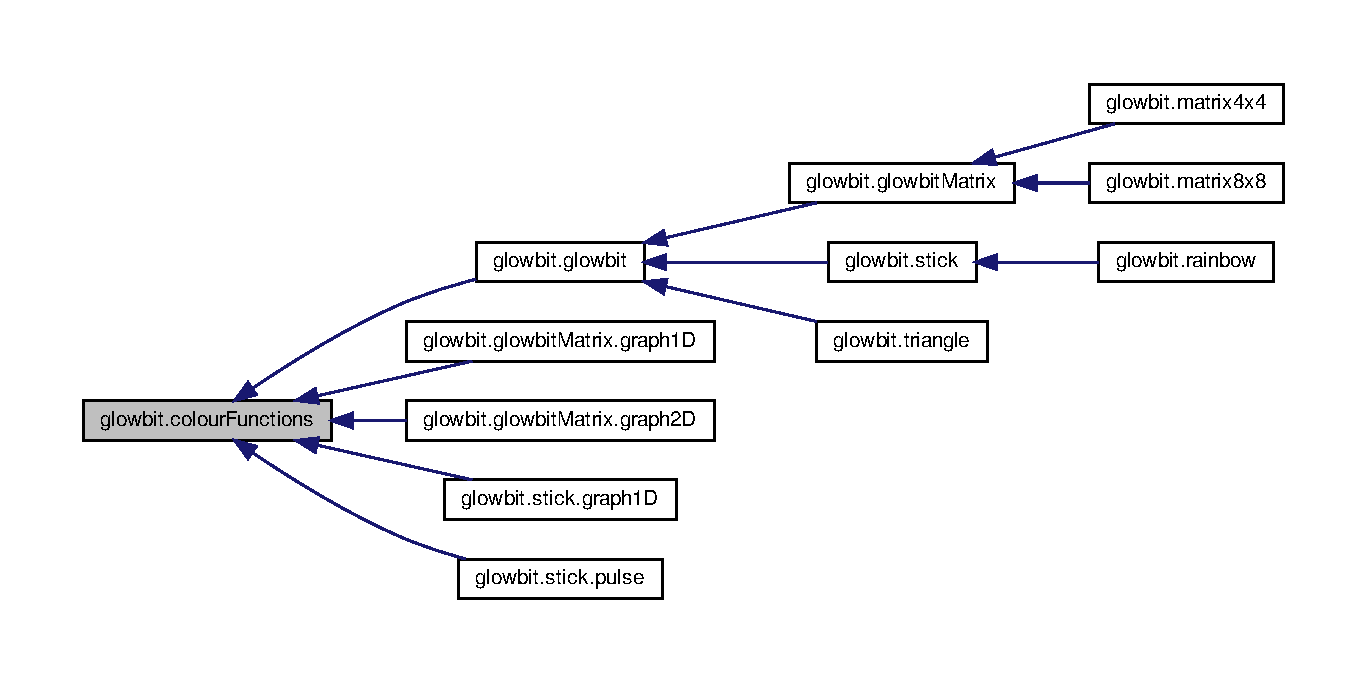
\includegraphics[width=350pt]{classglowbit_1_1colourFunctions__inherit__graph}
\end{center}
\end{figure}
\subsection*{Public Member Functions}
\begin{DoxyCompactItemize}
\item 
def \hyperlink{classglowbit_1_1colourFunctions_afb989958ec7aa4dfb7a04f359da5969a}{wheel} (self, pos)
\begin{DoxyCompactList}\small\item\em Converts an integer \char`\"{}colour wheel position\char`\"{} to a packed 32-\/bit R\+GB Glow\+Bit colour value. \end{DoxyCompactList}\item 
def \hyperlink{classglowbit_1_1colourFunctions_ad547ff80671bd310aac42051d81e6660}{rgb\+Colour} (self, r, g, b)
\begin{DoxyCompactList}\small\item\em Converts the r, g, and b integer arguments to a packed 32-\/bit R\+GB Glow\+Bit colour value. \end{DoxyCompactList}\item 
def \hyperlink{classglowbit_1_1colourFunctions_a6f887561ea3261440350ac3b1df4a259}{glowbit\+Colour2\+R\+GB} (self, colour)
\begin{DoxyCompactList}\small\item\em Converts a 32-\/bit Glow\+Bit colour value to an (R,G,B) tuple. \end{DoxyCompactList}\item 
\mbox{\Hypertarget{classglowbit_1_1colourFunctions_a409c07eda953f09150f4ba67111f14e4}\label{classglowbit_1_1colourFunctions_a409c07eda953f09150f4ba67111f14e4}} 
def \hyperlink{classglowbit_1_1colourFunctions_a409c07eda953f09150f4ba67111f14e4}{red} (self)
\begin{DoxyCompactList}\small\item\em Returns the Glow\+Bit colour value for pure red. \end{DoxyCompactList}\item 
\mbox{\Hypertarget{classglowbit_1_1colourFunctions_a822b37d8fa35cccd5ea9f2e0aa012435}\label{classglowbit_1_1colourFunctions_a822b37d8fa35cccd5ea9f2e0aa012435}} 
def \hyperlink{classglowbit_1_1colourFunctions_a822b37d8fa35cccd5ea9f2e0aa012435}{green} (self)
\begin{DoxyCompactList}\small\item\em Returns the Glow\+Bit colour value for pure green. \end{DoxyCompactList}\item 
\mbox{\Hypertarget{classglowbit_1_1colourFunctions_afe8c58ed88b15cb68fbd22e96c6ad51b}\label{classglowbit_1_1colourFunctions_afe8c58ed88b15cb68fbd22e96c6ad51b}} 
def \hyperlink{classglowbit_1_1colourFunctions_afe8c58ed88b15cb68fbd22e96c6ad51b}{blue} (self)
\begin{DoxyCompactList}\small\item\em Returns the Glow\+Bit colour value for pure blue. \end{DoxyCompactList}\item 
\mbox{\Hypertarget{classglowbit_1_1colourFunctions_a41f1916e8b9f6d14262ae7e37cfa47c3}\label{classglowbit_1_1colourFunctions_a41f1916e8b9f6d14262ae7e37cfa47c3}} 
def \hyperlink{classglowbit_1_1colourFunctions_a41f1916e8b9f6d14262ae7e37cfa47c3}{yellow} (self)
\begin{DoxyCompactList}\small\item\em Returns the Glow\+Bit colour value for yellow. \end{DoxyCompactList}\item 
\mbox{\Hypertarget{classglowbit_1_1colourFunctions_a1c476a787a727fc9bdc835ad75926e5d}\label{classglowbit_1_1colourFunctions_a1c476a787a727fc9bdc835ad75926e5d}} 
def \hyperlink{classglowbit_1_1colourFunctions_a1c476a787a727fc9bdc835ad75926e5d}{purple} (self)
\begin{DoxyCompactList}\small\item\em Returns the Glow\+Bit colour value for purple. \end{DoxyCompactList}\item 
\mbox{\Hypertarget{classglowbit_1_1colourFunctions_acbee8ca4dabce37aa663fbfbff2a3ae2}\label{classglowbit_1_1colourFunctions_acbee8ca4dabce37aa663fbfbff2a3ae2}} 
def \hyperlink{classglowbit_1_1colourFunctions_acbee8ca4dabce37aa663fbfbff2a3ae2}{cyan} (self)
\begin{DoxyCompactList}\small\item\em Returns the Glow\+Bit colour value for cyan. \end{DoxyCompactList}\item 
\mbox{\Hypertarget{classglowbit_1_1colourFunctions_a0c4d0695b48f4e17347a9924041ade59}\label{classglowbit_1_1colourFunctions_a0c4d0695b48f4e17347a9924041ade59}} 
def \hyperlink{classglowbit_1_1colourFunctions_a0c4d0695b48f4e17347a9924041ade59}{white} (self)
\begin{DoxyCompactList}\small\item\em Returns the Glow\+Bit colour value for white. \end{DoxyCompactList}\item 
\mbox{\Hypertarget{classglowbit_1_1colourFunctions_a3abddf433293e05d99d8c82309a08d41}\label{classglowbit_1_1colourFunctions_a3abddf433293e05d99d8c82309a08d41}} 
def \hyperlink{classglowbit_1_1colourFunctions_a3abddf433293e05d99d8c82309a08d41}{black} (self)
\begin{DoxyCompactList}\small\item\em Returns the Glow\+Bit colour value for black. \end{DoxyCompactList}\end{DoxyCompactItemize}


\subsection{Detailed Description}
Methods for transforming colours to 32-\/bit packed Glow\+Bit colour values. 

A packed 32-\/bit Glow\+Bit colour is an integer with 8-\/bits per colour channel data encoded in hexadecimal as follows\+:

0x00\+R\+R\+G\+G\+BB

where RR, GG, and BB are hexadecimal values (decimal \mbox{[}0,255\mbox{]}) and the most significant 8 bits are reserved and left as zero. 

\subsection{Member Function Documentation}
\mbox{\Hypertarget{classglowbit_1_1colourFunctions_a6f887561ea3261440350ac3b1df4a259}\label{classglowbit_1_1colourFunctions_a6f887561ea3261440350ac3b1df4a259}} 
\index{glowbit\+::colour\+Functions@{glowbit\+::colour\+Functions}!glowbit\+Colour2\+R\+GB@{glowbit\+Colour2\+R\+GB}}
\index{glowbit\+Colour2\+R\+GB@{glowbit\+Colour2\+R\+GB}!glowbit\+::colour\+Functions@{glowbit\+::colour\+Functions}}
\subsubsection{\texorpdfstring{glowbit\+Colour2\+R\+G\+B()}{glowbitColour2RGB()}}
{\footnotesize\ttfamily def glowbit.\+colour\+Functions.\+glowbit\+Colour2\+R\+GB (\begin{DoxyParamCaption}\item[{}]{self,  }\item[{}]{colour }\end{DoxyParamCaption})}



Converts a 32-\/bit Glow\+Bit colour value to an (R,G,B) tuple. 


\begin{DoxyParams}{Parameters}
{\em colour} & A 32-\/bit Glow\+Bit colour value \\
\hline
\end{DoxyParams}
\begin{DoxyReturn}{Returns}
A tuple in the format (R,G,B) containing the R\+GB components of the colour parameter 
\end{DoxyReturn}
\mbox{\Hypertarget{classglowbit_1_1colourFunctions_ad547ff80671bd310aac42051d81e6660}\label{classglowbit_1_1colourFunctions_ad547ff80671bd310aac42051d81e6660}} 
\index{glowbit\+::colour\+Functions@{glowbit\+::colour\+Functions}!rgb\+Colour@{rgb\+Colour}}
\index{rgb\+Colour@{rgb\+Colour}!glowbit\+::colour\+Functions@{glowbit\+::colour\+Functions}}
\subsubsection{\texorpdfstring{rgb\+Colour()}{rgbColour()}}
{\footnotesize\ttfamily def glowbit.\+colour\+Functions.\+rgb\+Colour (\begin{DoxyParamCaption}\item[{}]{self,  }\item[{}]{r,  }\item[{}]{g,  }\item[{}]{b }\end{DoxyParamCaption})}



Converts the r, g, and b integer arguments to a packed 32-\/bit R\+GB Glow\+Bit colour value. 

All arguments are required as this is a micropython viper function.


\begin{DoxyParams}{Parameters}
{\em r} & The red intensity, \mbox{[}0,255\mbox{]} \\
\hline
{\em g} & The green intensity, \mbox{[}0,255\mbox{]} \\
\hline
{\em b} & The blue intensity, \mbox{[}0,255\mbox{]} \\
\hline
\end{DoxyParams}
\begin{DoxyReturn}{Returns}
Packed 32-\/bit Glow\+Bit colour value 
\end{DoxyReturn}
\mbox{\Hypertarget{classglowbit_1_1colourFunctions_afb989958ec7aa4dfb7a04f359da5969a}\label{classglowbit_1_1colourFunctions_afb989958ec7aa4dfb7a04f359da5969a}} 
\index{glowbit\+::colour\+Functions@{glowbit\+::colour\+Functions}!wheel@{wheel}}
\index{wheel@{wheel}!glowbit\+::colour\+Functions@{glowbit\+::colour\+Functions}}
\subsubsection{\texorpdfstring{wheel()}{wheel()}}
{\footnotesize\ttfamily def glowbit.\+colour\+Functions.\+wheel (\begin{DoxyParamCaption}\item[{}]{self,  }\item[{}]{pos }\end{DoxyParamCaption})}



Converts an integer \char`\"{}colour wheel position\char`\"{} to a packed 32-\/bit R\+GB Glow\+Bit colour value. 

The \char`\"{}pos\char`\"{} argument is required as this is a micropython viper function.


\begin{DoxyParams}{Parameters}
{\em pos} & Colour wheel position \mbox{[}0,255\mbox{]} is mapped to a pure hue in the R\+GB colourspace. A value of 0 or 255 is mapped to pure red with a smooth red-\/yellow-\/green-\/blue-\/purple-\/magenta-\/red transion for other values. \\
\hline
\end{DoxyParams}
\begin{DoxyReturn}{Returns}
32-\/bit integer Glow\+Bit colour value 
\end{DoxyReturn}


The documentation for this class was generated from the following file\+:\begin{DoxyCompactItemize}
\item 
glowbit.\+py\end{DoxyCompactItemize}

\hypertarget{classglowbit_1_1colourMaps}{}\section{glowbit.\+colour\+Maps Class Reference}
\label{classglowbit_1_1colourMaps}\index{glowbit.\+colour\+Maps@{glowbit.\+colour\+Maps}}


Methods which calculate colour gradients.  




Inheritance diagram for glowbit.\+colour\+Maps\+:\nopagebreak
\begin{figure}[H]
\begin{center}
\leavevmode
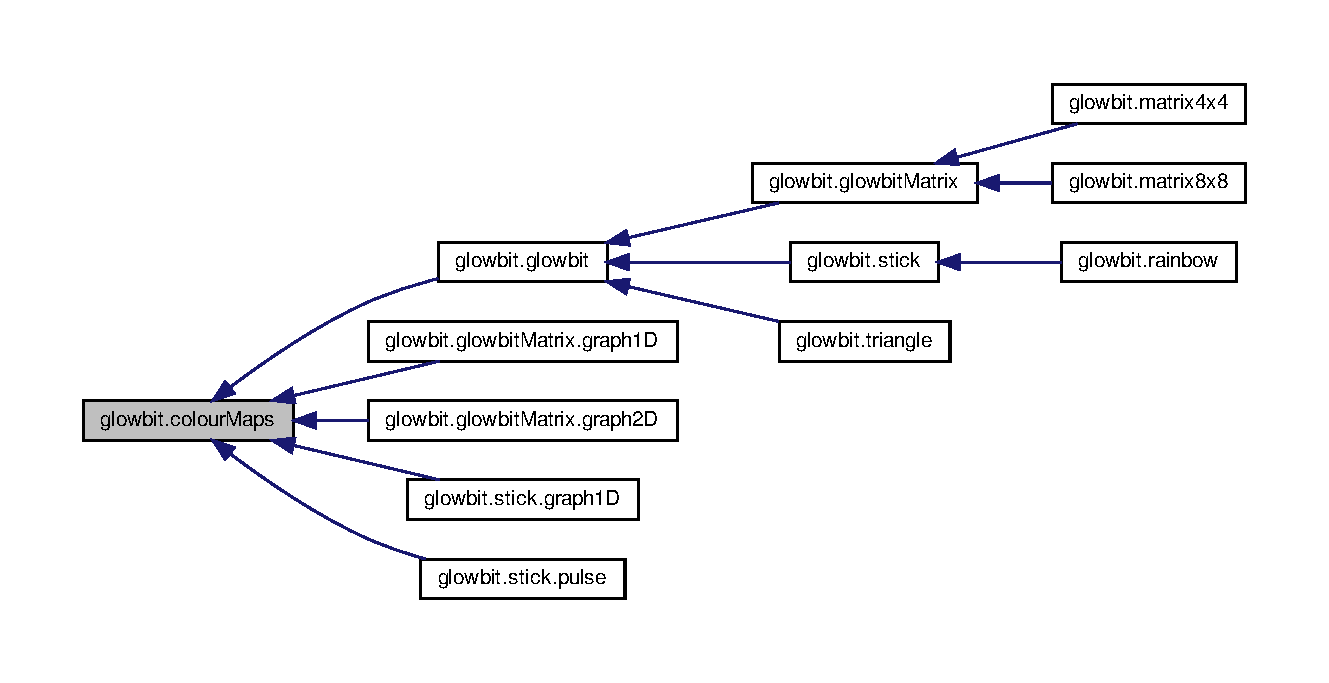
\includegraphics[width=350pt]{classglowbit_1_1colourMaps__inherit__graph}
\end{center}
\end{figure}
\subsection*{Public Member Functions}
\begin{DoxyCompactItemize}
\item 
def \hyperlink{classglowbit_1_1colourMaps_ab54dfebabe1485e9cf2a9d47e6df24a1}{colour\+Map\+Solid} (self, index, min\+Index, max\+Index)
\begin{DoxyCompactList}\small\item\em Trivial colourmap method which always returns the colour in the parent object. \end{DoxyCompactList}\item 
def \hyperlink{classglowbit_1_1colourMaps_a41e8852322605003cf7f9f75ff508a8e}{colour\+Map\+Rainbow} (self, index, min\+Index, max\+Index)
\begin{DoxyCompactList}\small\item\em Maps the pure hue colour wheel between min\+Index and max\+Index. \end{DoxyCompactList}\end{DoxyCompactItemize}


\subsection{Detailed Description}
Methods which calculate colour gradients. 

Custom colour map methods can be written and passed to several Glow\+Bit library methods (eg\+: \hyperlink{classglowbit_1_1stick_1_1graph1D}{glowbit.\+stick.\+graph1D}) but must accept the same positional arguments as the methods in this class\+:

def colour\+Map\+Function(self, index, min\+Index, max\+Index)\+: 

\subsection{Member Function Documentation}
\mbox{\Hypertarget{classglowbit_1_1colourMaps_a41e8852322605003cf7f9f75ff508a8e}\label{classglowbit_1_1colourMaps_a41e8852322605003cf7f9f75ff508a8e}} 
\index{glowbit\+::colour\+Maps@{glowbit\+::colour\+Maps}!colour\+Map\+Rainbow@{colour\+Map\+Rainbow}}
\index{colour\+Map\+Rainbow@{colour\+Map\+Rainbow}!glowbit\+::colour\+Maps@{glowbit\+::colour\+Maps}}
\subsubsection{\texorpdfstring{colour\+Map\+Rainbow()}{colourMapRainbow()}}
{\footnotesize\ttfamily def glowbit.\+colour\+Maps.\+colour\+Map\+Rainbow (\begin{DoxyParamCaption}\item[{}]{self,  }\item[{}]{index,  }\item[{}]{min\+Index,  }\item[{}]{max\+Index }\end{DoxyParamCaption})}



Maps the pure hue colour wheel between min\+Index and max\+Index. 


\begin{DoxyParams}{Parameters}
{\em index} & The value to be mapped \\
\hline
{\em min\+Index} & The value of index mapped to a colour wheel angle of 0 degrees \\
\hline
{\em max\+Index} & The value of index mapped to a colour wheel angle of 360 degrees \\
\hline
\end{DoxyParams}
\begin{DoxyReturn}{Returns}
The 32-\/bit packed Glow\+Bit colour value 
\end{DoxyReturn}
\mbox{\Hypertarget{classglowbit_1_1colourMaps_ab54dfebabe1485e9cf2a9d47e6df24a1}\label{classglowbit_1_1colourMaps_ab54dfebabe1485e9cf2a9d47e6df24a1}} 
\index{glowbit\+::colour\+Maps@{glowbit\+::colour\+Maps}!colour\+Map\+Solid@{colour\+Map\+Solid}}
\index{colour\+Map\+Solid@{colour\+Map\+Solid}!glowbit\+::colour\+Maps@{glowbit\+::colour\+Maps}}
\subsubsection{\texorpdfstring{colour\+Map\+Solid()}{colourMapSolid()}}
{\footnotesize\ttfamily def glowbit.\+colour\+Maps.\+colour\+Map\+Solid (\begin{DoxyParamCaption}\item[{}]{self,  }\item[{}]{index,  }\item[{}]{min\+Index,  }\item[{}]{max\+Index }\end{DoxyParamCaption})}



Trivial colourmap method which always returns the colour in the parent object. 


\begin{DoxyParams}{Parameters}
{\em index} & Dummy argument for compatibility with colourmap method A\+PI \\
\hline
{\em min\+Index} & Dummy argument for compatibility with colourmap method A\+PI \\
\hline
{\em max\+Index} & Dummy argument for compatibility with colourmap method A\+PI \\
\hline
\end{DoxyParams}


The documentation for this class was generated from the following file\+:\begin{DoxyCompactItemize}
\item 
glowbit.\+py\end{DoxyCompactItemize}

\hypertarget{classglowbit_1_1glowbit}{}\section{glowbit.\+glowbit Class Reference}
\label{classglowbit_1_1glowbit}\index{glowbit.\+glowbit@{glowbit.\+glowbit}}


Low-\/level methods common to all Glow\+Bit classes.  




Inheritance diagram for glowbit.\+glowbit\+:\nopagebreak
\begin{figure}[H]
\begin{center}
\leavevmode
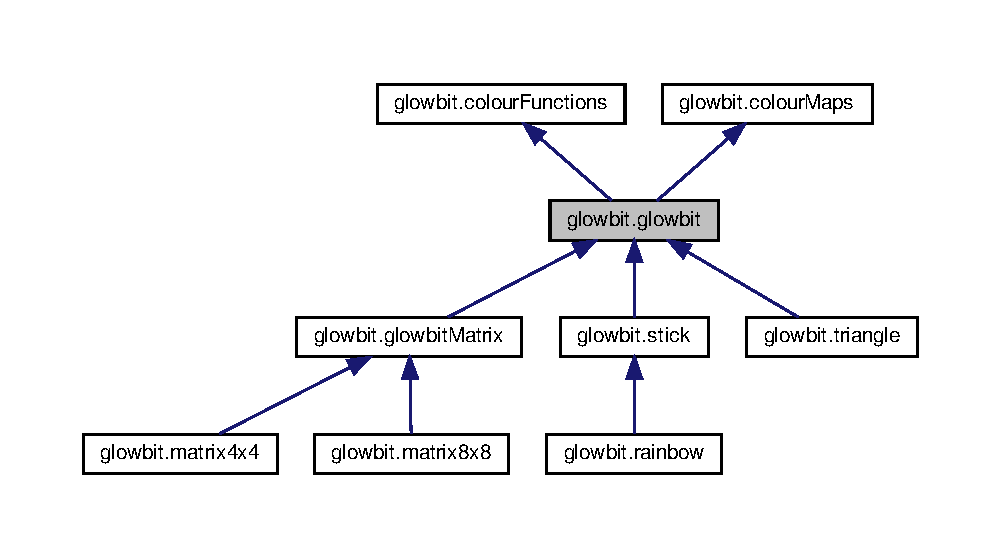
\includegraphics[width=350pt]{classglowbit_1_1glowbit__inherit__graph}
\end{center}
\end{figure}


Collaboration diagram for glowbit.\+glowbit\+:\nopagebreak
\begin{figure}[H]
\begin{center}
\leavevmode
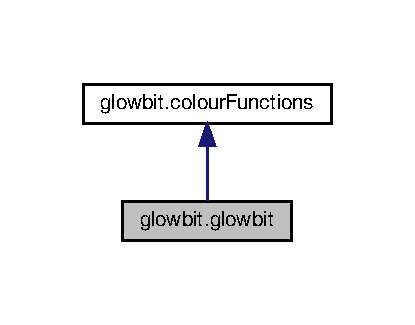
\includegraphics[width=199pt]{classglowbit_1_1glowbit__coll__graph}
\end{center}
\end{figure}
\subsection*{Public Member Functions}
\begin{DoxyCompactItemize}
\item 
def \hyperlink{classglowbit_1_1glowbit_a051aed2a4969fdcb0466e4e840209279}{pixels\+Show} (self)
\begin{DoxyCompactList}\small\item\em Pushes the internal pixel data buffer to the physical Glow\+Bit L\+E\+Ds. \end{DoxyCompactList}\item 
def \hyperlink{classglowbit_1_1glowbit_a6184de87721652f9f55f9301f6a3a9ce}{pixel\+Set} (self, i, colour)
\begin{DoxyCompactList}\small\item\em Sets the i\textquotesingle{}th Glow\+Bit L\+ED to a 32-\/bit Glow\+Bit colour value. \end{DoxyCompactList}\item 
def \hyperlink{classglowbit_1_1glowbit_a6f4167e566106d5eb104933b256f2e14}{pixel\+Set\+Now} (self, i, colour)
\begin{DoxyCompactList}\small\item\em Sets the i\textquotesingle{}th Glow\+Bit L\+ED to a 32-\/bit Glow\+Bit colour value and updates the physical L\+E\+Ds. \end{DoxyCompactList}\item 
def \hyperlink{classglowbit_1_1glowbit_a8bb7ba36b4b7746f215ebad1acc0f5e2}{pixel\+Add} (self, i, colour)
\begin{DoxyCompactList}\small\item\em Adds a 32-\/bit Glow\+Bit colour value to the i\textquotesingle{}th L\+ED in the internal buffer only. \end{DoxyCompactList}\item 
def \hyperlink{classglowbit_1_1glowbit_aca86823fecc4949692ac18f8c21e34ac}{pixels\+Fill} (self, colour)
\begin{DoxyCompactList}\small\item\em Fills all pixels with a solid colour value. \end{DoxyCompactList}\item 
def \hyperlink{classglowbit_1_1glowbit_a2aae728fcc6e8cdfe5c745ac0a7d308d}{pixels\+Fill\+Now} (self, colour)
\begin{DoxyCompactList}\small\item\em Fills all pixels with a solid colour value and updates the physical L\+E\+Ds. \end{DoxyCompactList}\item 
def \hyperlink{classglowbit_1_1glowbit_ad3ace3e4d58bc9dadf62c1306aff2464}{blank\+Display} (self)
\begin{DoxyCompactList}\small\item\em Blanks the entire Glow\+Bit display. \end{DoxyCompactList}\item 
\mbox{\Hypertarget{classglowbit_1_1glowbit_a0f15a8907f807ed1af905854fedbbc60}\label{classglowbit_1_1glowbit_a0f15a8907f807ed1af905854fedbbc60}} 
def {\bfseries get\+Pixel} (self, N)
\item 
\mbox{\Hypertarget{classglowbit_1_1glowbit_a7f72cb0878a688aa6181d4632428da09}\label{classglowbit_1_1glowbit_a7f72cb0878a688aa6181d4632428da09}} 
def {\bfseries update\+Rate\+Limit\+F\+PS} (self, rate\+Limit\+F\+PS)
\item 
\mbox{\Hypertarget{classglowbit_1_1glowbit_ae95bb7e0ee556e02d918f376cffcb9ce}\label{classglowbit_1_1glowbit_ae95bb7e0ee556e02d918f376cffcb9ce}} 
def {\bfseries chaos} (self, iters=100)
\end{DoxyCompactItemize}
\subsection*{Public Attributes}
\begin{DoxyCompactItemize}
\item 
\mbox{\Hypertarget{classglowbit_1_1glowbit_a5f14ddb9b3ec9a848c050b28d27ced9e}\label{classglowbit_1_1glowbit_a5f14ddb9b3ec9a848c050b28d27ced9e}} 
{\bfseries last\+Frame\+\_\+ms}
\item 
\mbox{\Hypertarget{classglowbit_1_1glowbit_a69bf20e5a054c0cf8656986b07048851}\label{classglowbit_1_1glowbit_a69bf20e5a054c0cf8656986b07048851}} 
{\bfseries rate\+Limit}
\end{DoxyCompactItemize}
\subsection*{Static Public Attributes}
\begin{DoxyCompactItemize}
\item 
\mbox{\Hypertarget{classglowbit_1_1glowbit_a73c5457f4f8442a9ba5fdaa0cd7ea4b5}\label{classglowbit_1_1glowbit_a73c5457f4f8442a9ba5fdaa0cd7ea4b5}} 
{\bfseries sideset\+\_\+init}
\item 
\mbox{\Hypertarget{classglowbit_1_1glowbit_a1ed8a1be31b4b872d9ccb7ac5e30892d}\label{classglowbit_1_1glowbit_a1ed8a1be31b4b872d9ccb7ac5e30892d}} 
{\bfseries O\+U\+T\+\_\+\+L\+OW}
\item 
\mbox{\Hypertarget{classglowbit_1_1glowbit_a15cd9fc87ac01180b047877394d0c002}\label{classglowbit_1_1glowbit_a15cd9fc87ac01180b047877394d0c002}} 
{\bfseries out\+\_\+shiftdir}
\item 
\mbox{\Hypertarget{classglowbit_1_1glowbit_a60284b74a652f430dbdde8e16a6c05a1}\label{classglowbit_1_1glowbit_a60284b74a652f430dbdde8e16a6c05a1}} 
{\bfseries S\+H\+I\+F\+T\+\_\+\+L\+E\+FT}
\item 
\mbox{\Hypertarget{classglowbit_1_1glowbit_ae34f402180e4f4ec9a050b737504f078}\label{classglowbit_1_1glowbit_ae34f402180e4f4ec9a050b737504f078}} 
{\bfseries autopull}
\item 
\mbox{\Hypertarget{classglowbit_1_1glowbit_a09fe7452d85b7fed1f154c22f125b6c7}\label{classglowbit_1_1glowbit_a09fe7452d85b7fed1f154c22f125b6c7}} 
{\bfseries True}
\item 
\mbox{\Hypertarget{classglowbit_1_1glowbit_ae08d4038b7463323e58b07c4020d484d}\label{classglowbit_1_1glowbit_ae08d4038b7463323e58b07c4020d484d}} 
{\bfseries pull\+\_\+thresh}
\end{DoxyCompactItemize}


\subsection{Detailed Description}
Low-\/level methods common to all Glow\+Bit classes. 

\subsection{Member Function Documentation}
\mbox{\Hypertarget{classglowbit_1_1glowbit_ad3ace3e4d58bc9dadf62c1306aff2464}\label{classglowbit_1_1glowbit_ad3ace3e4d58bc9dadf62c1306aff2464}} 
\index{glowbit\+::glowbit@{glowbit\+::glowbit}!blank\+Display@{blank\+Display}}
\index{blank\+Display@{blank\+Display}!glowbit\+::glowbit@{glowbit\+::glowbit}}
\subsubsection{\texorpdfstring{blank\+Display()}{blankDisplay()}}
{\footnotesize\ttfamily def glowbit.\+glowbit.\+blank\+Display (\begin{DoxyParamCaption}\item[{}]{self }\end{DoxyParamCaption})}



Blanks the entire Glow\+Bit display. 

ie\+: sets the colour value of all Glow\+Bit L\+E\+Ds to zero in the internal buffer and updates the physical L\+E\+Ds. \mbox{\Hypertarget{classglowbit_1_1glowbit_a8bb7ba36b4b7746f215ebad1acc0f5e2}\label{classglowbit_1_1glowbit_a8bb7ba36b4b7746f215ebad1acc0f5e2}} 
\index{glowbit\+::glowbit@{glowbit\+::glowbit}!pixel\+Add@{pixel\+Add}}
\index{pixel\+Add@{pixel\+Add}!glowbit\+::glowbit@{glowbit\+::glowbit}}
\subsubsection{\texorpdfstring{pixel\+Add()}{pixelAdd()}}
{\footnotesize\ttfamily def glowbit.\+glowbit.\+pixel\+Add (\begin{DoxyParamCaption}\item[{}]{self,  }\item[{}]{i,  }\item[{}]{colour }\end{DoxyParamCaption})}



Adds a 32-\/bit Glow\+Bit colour value to the i\textquotesingle{}th L\+ED in the internal buffer only. 

Data colour corruption will occur if the sum result of any R\+GB value exceeds 255. Care must be taken to avoid this manually. eg\+: if the blue channel\textquotesingle{}s resulting intensity value is 256 it will be set to zero and the red channel incremented by 1. See the \hyperlink{classglowbit_1_1colourFunctions}{colour\+Functions} class documentation for the 32-\/bit Glow\+Bit colour specification.

NB\+: For efficiency, this method does not do any index bounds checking. If the value of the parameter i is larger than the number of L\+E\+Ds it will cause an Index\+Error exception.


\begin{DoxyParams}{Parameters}
{\em i} & An L\+ED\textquotesingle{}s index \\
\hline
{\em colour} & The 32-\/bit Glow\+Bit colour value \\
\hline
\end{DoxyParams}
\mbox{\Hypertarget{classglowbit_1_1glowbit_a6184de87721652f9f55f9301f6a3a9ce}\label{classglowbit_1_1glowbit_a6184de87721652f9f55f9301f6a3a9ce}} 
\index{glowbit\+::glowbit@{glowbit\+::glowbit}!pixel\+Set@{pixel\+Set}}
\index{pixel\+Set@{pixel\+Set}!glowbit\+::glowbit@{glowbit\+::glowbit}}
\subsubsection{\texorpdfstring{pixel\+Set()}{pixelSet()}}
{\footnotesize\ttfamily def glowbit.\+glowbit.\+pixel\+Set (\begin{DoxyParamCaption}\item[{}]{self,  }\item[{}]{i,  }\item[{}]{colour }\end{DoxyParamCaption})}



Sets the i\textquotesingle{}th Glow\+Bit L\+ED to a 32-\/bit Glow\+Bit colour value. 

NB\+: For efficiency, this method does not do any bounds checking. If the value of the parameter i is larger than the number of L\+E\+Ds it will cause an Index\+Error exception.


\begin{DoxyParams}{Parameters}
{\em i} & An L\+ED\textquotesingle{}s index \\
\hline
{\em colour} & The 32-\/bit Glow\+Bit colour value \\
\hline
\end{DoxyParams}
\mbox{\Hypertarget{classglowbit_1_1glowbit_a6f4167e566106d5eb104933b256f2e14}\label{classglowbit_1_1glowbit_a6f4167e566106d5eb104933b256f2e14}} 
\index{glowbit\+::glowbit@{glowbit\+::glowbit}!pixel\+Set\+Now@{pixel\+Set\+Now}}
\index{pixel\+Set\+Now@{pixel\+Set\+Now}!glowbit\+::glowbit@{glowbit\+::glowbit}}
\subsubsection{\texorpdfstring{pixel\+Set\+Now()}{pixelSetNow()}}
{\footnotesize\ttfamily def glowbit.\+glowbit.\+pixel\+Set\+Now (\begin{DoxyParamCaption}\item[{}]{self,  }\item[{}]{i,  }\item[{}]{colour }\end{DoxyParamCaption})}



Sets the i\textquotesingle{}th Glow\+Bit L\+ED to a 32-\/bit Glow\+Bit colour value and updates the physical L\+E\+Ds. 

NB\+: For efficiency, this method does not do any index bounds checking. If the value of the parameter i is larger than the number of L\+E\+Ds it will cause an Index\+Error exception.


\begin{DoxyParams}{Parameters}
{\em i} & An L\+ED\textquotesingle{}s index \\
\hline
{\em colour} & The 32-\/bit Glow\+Bit colour value \\
\hline
\end{DoxyParams}
\mbox{\Hypertarget{classglowbit_1_1glowbit_aca86823fecc4949692ac18f8c21e34ac}\label{classglowbit_1_1glowbit_aca86823fecc4949692ac18f8c21e34ac}} 
\index{glowbit\+::glowbit@{glowbit\+::glowbit}!pixels\+Fill@{pixels\+Fill}}
\index{pixels\+Fill@{pixels\+Fill}!glowbit\+::glowbit@{glowbit\+::glowbit}}
\subsubsection{\texorpdfstring{pixels\+Fill()}{pixelsFill()}}
{\footnotesize\ttfamily def glowbit.\+glowbit.\+pixels\+Fill (\begin{DoxyParamCaption}\item[{}]{self,  }\item[{}]{colour }\end{DoxyParamCaption})}



Fills all pixels with a solid colour value. 


\begin{DoxyParams}{Parameters}
{\em colour} & The 32-\/bit Glow\+Bit colour value \\
\hline
\end{DoxyParams}
\mbox{\Hypertarget{classglowbit_1_1glowbit_a2aae728fcc6e8cdfe5c745ac0a7d308d}\label{classglowbit_1_1glowbit_a2aae728fcc6e8cdfe5c745ac0a7d308d}} 
\index{glowbit\+::glowbit@{glowbit\+::glowbit}!pixels\+Fill\+Now@{pixels\+Fill\+Now}}
\index{pixels\+Fill\+Now@{pixels\+Fill\+Now}!glowbit\+::glowbit@{glowbit\+::glowbit}}
\subsubsection{\texorpdfstring{pixels\+Fill\+Now()}{pixelsFillNow()}}
{\footnotesize\ttfamily def glowbit.\+glowbit.\+pixels\+Fill\+Now (\begin{DoxyParamCaption}\item[{}]{self,  }\item[{}]{colour }\end{DoxyParamCaption})}



Fills all pixels with a solid colour value and updates the physical L\+E\+Ds. 


\begin{DoxyParams}{Parameters}
{\em colour} & The 32-\/bit Glow\+Bit colour value \\
\hline
\end{DoxyParams}
\mbox{\Hypertarget{classglowbit_1_1glowbit_a051aed2a4969fdcb0466e4e840209279}\label{classglowbit_1_1glowbit_a051aed2a4969fdcb0466e4e840209279}} 
\index{glowbit\+::glowbit@{glowbit\+::glowbit}!pixels\+Show@{pixels\+Show}}
\index{pixels\+Show@{pixels\+Show}!glowbit\+::glowbit@{glowbit\+::glowbit}}
\subsubsection{\texorpdfstring{pixels\+Show()}{pixelsShow()}}
{\footnotesize\ttfamily def glowbit.\+glowbit.\+pixels\+Show (\begin{DoxyParamCaption}\item[{}]{self }\end{DoxyParamCaption})}



Pushes the internal pixel data buffer to the physical Glow\+Bit L\+E\+Ds. 

This function must be called before the connected Glow\+Bit L\+E\+Ds will change colour.

Note that several Glow\+Bit library methods call this method unconditionally (eg\+: blank\+Display ) or optionally (eg\+: by passing the update = True parameter to stick.\+graph1\+D() ) 

The documentation for this class was generated from the following file\+:\begin{DoxyCompactItemize}
\item 
glowbit.\+py\end{DoxyCompactItemize}

\hypertarget{classglowbit_1_1glowbitMatrix}{}\section{glowbit.\+glowbit\+Matrix Class Reference}
\label{classglowbit_1_1glowbitMatrix}\index{glowbit.\+glowbit\+Matrix@{glowbit.\+glowbit\+Matrix}}


Inheritance diagram for glowbit.\+glowbit\+Matrix\+:\nopagebreak
\begin{figure}[H]
\begin{center}
\leavevmode
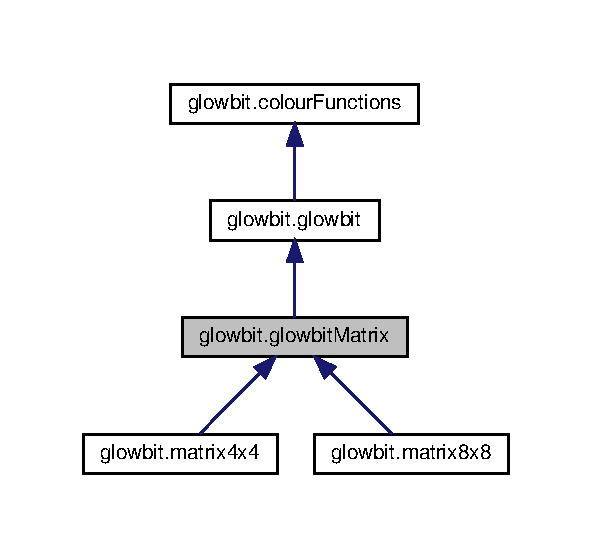
\includegraphics[width=284pt]{classglowbit_1_1glowbitMatrix__inherit__graph}
\end{center}
\end{figure}


Collaboration diagram for glowbit.\+glowbit\+Matrix\+:\nopagebreak
\begin{figure}[H]
\begin{center}
\leavevmode
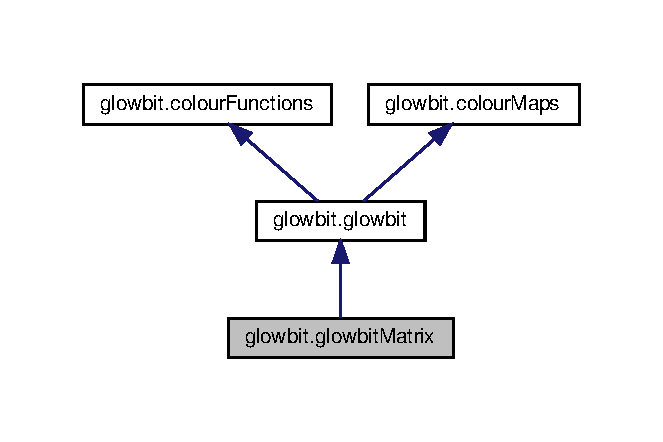
\includegraphics[width=199pt]{classglowbit_1_1glowbitMatrix__coll__graph}
\end{center}
\end{figure}
\subsection*{Classes}
\begin{DoxyCompactItemize}
\item 
class \hyperlink{classglowbit_1_1glowbitMatrix_1_1graph1D}{graph1D}
\item 
class \hyperlink{classglowbit_1_1glowbitMatrix_1_1graph2D}{graph2D}
\item 
class \hyperlink{classglowbit_1_1glowbitMatrix_1_1raindrop}{raindrop}
\end{DoxyCompactItemize}
\subsection*{Public Member Functions}
\begin{DoxyCompactItemize}
\item 
\mbox{\Hypertarget{classglowbit_1_1glowbitMatrix_a5f20884e1b08bc66e54860d0bbf0d22e}\label{classglowbit_1_1glowbitMatrix_a5f20884e1b08bc66e54860d0bbf0d22e}} 
def {\bfseries pixel\+Set\+XY} (self, x, y, colour)
\item 
\mbox{\Hypertarget{classglowbit_1_1glowbitMatrix_ab100bb891bab3d6479b066049ce9a367}\label{classglowbit_1_1glowbitMatrix_ab100bb891bab3d6479b066049ce9a367}} 
def {\bfseries pixel\+Set\+X\+Y\+Now} (self, x, y, colour)
\item 
\mbox{\Hypertarget{classglowbit_1_1glowbitMatrix_af33f1952a94e2f0933386ae2e7c5bca4}\label{classglowbit_1_1glowbitMatrix_af33f1952a94e2f0933386ae2e7c5bca4}} 
def {\bfseries pixel\+Set\+X\+Y\+Clip} (self, x, y, colour)
\item 
\mbox{\Hypertarget{classglowbit_1_1glowbitMatrix_ae05d008c207c5f5219e737d29185501e}\label{classglowbit_1_1glowbitMatrix_ae05d008c207c5f5219e737d29185501e}} 
def {\bfseries pixel\+Add\+XY} (self, x, y, colour)
\item 
\mbox{\Hypertarget{classglowbit_1_1glowbitMatrix_a4f2deb5f58f45e285e84c9cac1644618}\label{classglowbit_1_1glowbitMatrix_a4f2deb5f58f45e285e84c9cac1644618}} 
def {\bfseries pixel\+Add\+X\+Y\+Clip} (self, x, y, colour)
\item 
\mbox{\Hypertarget{classglowbit_1_1glowbitMatrix_ab67885d63f392afa061c8455de3e31ba}\label{classglowbit_1_1glowbitMatrix_ab67885d63f392afa061c8455de3e31ba}} 
def {\bfseries get\+Pixel\+XY} (self, x, y)
\item 
\mbox{\Hypertarget{classglowbit_1_1glowbitMatrix_a373a7739051a7399a94636375ac0b4ec}\label{classglowbit_1_1glowbitMatrix_a373a7739051a7399a94636375ac0b4ec}} 
def {\bfseries draw\+Line} (self, x0, y0, x1, y1, colour)
\item 
\mbox{\Hypertarget{classglowbit_1_1glowbitMatrix_ac0b08486a62b6bd9c8633287d2725f43}\label{classglowbit_1_1glowbitMatrix_ac0b08486a62b6bd9c8633287d2725f43}} 
def {\bfseries draw\+Triangle} (self, x0, y0, x1, y1, x2, y2, colour)
\item 
\mbox{\Hypertarget{classglowbit_1_1glowbitMatrix_ad70235a976475054af4ccb534a32b5e7}\label{classglowbit_1_1glowbitMatrix_ad70235a976475054af4ccb534a32b5e7}} 
def {\bfseries draw\+Rectangle} (self, x0, y0, x1, y1, colour)
\item 
\mbox{\Hypertarget{classglowbit_1_1glowbitMatrix_ad91952585c61527ae5c0ac4a170435bf}\label{classglowbit_1_1glowbitMatrix_ad91952585c61527ae5c0ac4a170435bf}} 
def {\bfseries draw\+Rectangle\+Fill} (self, x0, y0, x1, y1, colour)
\item 
\mbox{\Hypertarget{classglowbit_1_1glowbitMatrix_a4efec5ce17c30403505b1f2775022e90}\label{classglowbit_1_1glowbitMatrix_a4efec5ce17c30403505b1f2775022e90}} 
def {\bfseries draw\+Circle} (self, x0, y0, r, colour)
\item 
\mbox{\Hypertarget{classglowbit_1_1glowbitMatrix_a0d44976cdc12728d9ae80c2d901029c0}\label{classglowbit_1_1glowbitMatrix_a0d44976cdc12728d9ae80c2d901029c0}} 
def {\bfseries update\+Graph1D} (self, graph, value)
\item 
\mbox{\Hypertarget{classglowbit_1_1glowbitMatrix_aaf5d23a0ed51901ffd78dfae985fbc7f}\label{classglowbit_1_1glowbitMatrix_aaf5d23a0ed51901ffd78dfae985fbc7f}} 
def {\bfseries update\+Graph2D} (self, graph)
\item 
\mbox{\Hypertarget{classglowbit_1_1glowbitMatrix_a0071fd8471e5f519586f6fdd86f8d7f3}\label{classglowbit_1_1glowbitMatrix_a0071fd8471e5f519586f6fdd86f8d7f3}} 
def {\bfseries line\+Demo} (self, iters=10)
\item 
\mbox{\Hypertarget{classglowbit_1_1glowbitMatrix_a69370ec1479b4887fca517fbefd92e4c}\label{classglowbit_1_1glowbitMatrix_a69370ec1479b4887fca517fbefd92e4c}} 
def {\bfseries fireworks} (self, iters=10)
\item 
\mbox{\Hypertarget{classglowbit_1_1glowbitMatrix_adf29bdb4294bcf27ae560130b0fcae35}\label{classglowbit_1_1glowbitMatrix_adf29bdb4294bcf27ae560130b0fcae35}} 
def {\bfseries circular\+Rainbow} (self)
\item 
\mbox{\Hypertarget{classglowbit_1_1glowbitMatrix_a690a172f923caeb55e3adf012ec0600c}\label{classglowbit_1_1glowbitMatrix_a690a172f923caeb55e3adf012ec0600c}} 
def {\bfseries rain} (self, iters=1000, density=1)
\item 
\mbox{\Hypertarget{classglowbit_1_1glowbitMatrix_a6232220b12c86c7ec361cde374419ac4}\label{classglowbit_1_1glowbitMatrix_a6232220b12c86c7ec361cde374419ac4}} 
def {\bfseries text\+Demo} (self, text=\char`\"{}Scrolling Text Demo\char`\"{})
\item 
\mbox{\Hypertarget{classglowbit_1_1glowbitMatrix_a969352871a02db3d55bcabe5b5107574}\label{classglowbit_1_1glowbitMatrix_a969352871a02db3d55bcabe5b5107574}} 
def {\bfseries bounce} (self, iters=1000)
\end{DoxyCompactItemize}
\subsection*{Additional Inherited Members}


The documentation for this class was generated from the following file\+:\begin{DoxyCompactItemize}
\item 
glowbit.\+py\end{DoxyCompactItemize}

\hypertarget{classglowbit_1_1glowbitMatrix_1_1graph1D}{}\section{glowbit.\+glowbit\+Matrix.\+graph1D Class Reference}
\label{classglowbit_1_1glowbitMatrix_1_1graph1D}\index{glowbit.\+glowbit\+Matrix.\+graph1D@{glowbit.\+glowbit\+Matrix.\+graph1D}}


Inheritance diagram for glowbit.\+glowbit\+Matrix.\+graph1D\+:\nopagebreak
\begin{figure}[H]
\begin{center}
\leavevmode
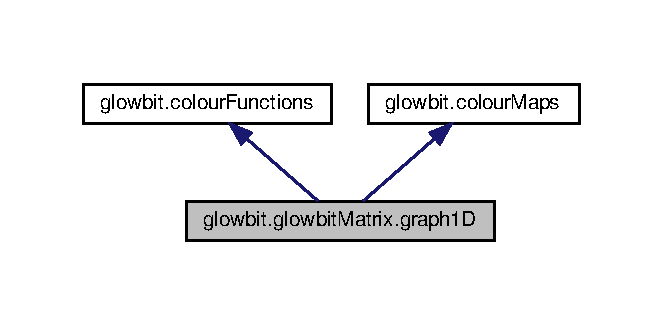
\includegraphics[width=318pt]{classglowbit_1_1glowbitMatrix_1_1graph1D__inherit__graph}
\end{center}
\end{figure}


Collaboration diagram for glowbit.\+glowbit\+Matrix.\+graph1D\+:\nopagebreak
\begin{figure}[H]
\begin{center}
\leavevmode
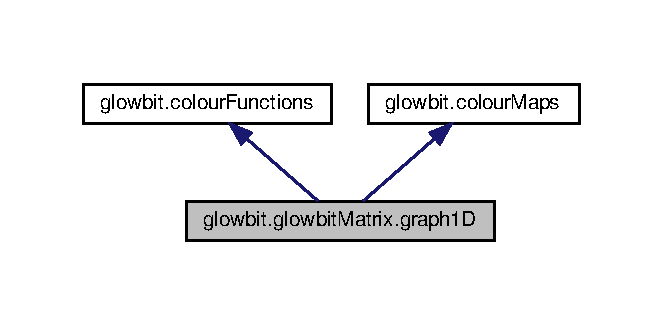
\includegraphics[width=318pt]{classglowbit_1_1glowbitMatrix_1_1graph1D__coll__graph}
\end{center}
\end{figure}
\subsection*{Public Member Functions}
\begin{DoxyCompactItemize}
\item 
\mbox{\Hypertarget{classglowbit_1_1glowbitMatrix_1_1graph1D_aafb789a57fe97ce1625bfb486400b2a1}\label{classglowbit_1_1glowbitMatrix_1_1graph1D_aafb789a57fe97ce1625bfb486400b2a1}} 
def {\bfseries \+\_\+\+\_\+init\+\_\+\+\_\+} (self, originX=0, originY=7, length=8, direction=\char`\"{}Up\char`\"{}, min\+Value=0, max\+Value=255, colour=0x\+F\+F\+F\+F\+F\+F, colour\+Map=\char`\"{}\+Solid\char`\"{}, update=\+False)
\end{DoxyCompactItemize}
\subsection*{Public Attributes}
\begin{DoxyCompactItemize}
\item 
\mbox{\Hypertarget{classglowbit_1_1glowbitMatrix_1_1graph1D_aa3d020bb8aa07dfb208582b045fc0c27}\label{classglowbit_1_1glowbitMatrix_1_1graph1D_aa3d020bb8aa07dfb208582b045fc0c27}} 
{\bfseries min\+Value}
\item 
\mbox{\Hypertarget{classglowbit_1_1glowbitMatrix_1_1graph1D_ab4d267a5d54ee085f3d9730111793dee}\label{classglowbit_1_1glowbitMatrix_1_1graph1D_ab4d267a5d54ee085f3d9730111793dee}} 
{\bfseries max\+Value}
\item 
\mbox{\Hypertarget{classglowbit_1_1glowbitMatrix_1_1graph1D_abe80fa374ef4be3d221174f6184c5ae4}\label{classglowbit_1_1glowbitMatrix_1_1graph1D_abe80fa374ef4be3d221174f6184c5ae4}} 
{\bfseries originX}
\item 
\mbox{\Hypertarget{classglowbit_1_1glowbitMatrix_1_1graph1D_aa72de1eb6177af6f741c2e298bd890f6}\label{classglowbit_1_1glowbitMatrix_1_1graph1D_aa72de1eb6177af6f741c2e298bd890f6}} 
{\bfseries originY}
\item 
\mbox{\Hypertarget{classglowbit_1_1glowbitMatrix_1_1graph1D_a1b650cb2675d638268381e8a07fe6533}\label{classglowbit_1_1glowbitMatrix_1_1graph1D_a1b650cb2675d638268381e8a07fe6533}} 
{\bfseries length}
\item 
\mbox{\Hypertarget{classglowbit_1_1glowbitMatrix_1_1graph1D_acd0f6e12bc30ce6f111cb6eaae9ef24e}\label{classglowbit_1_1glowbitMatrix_1_1graph1D_acd0f6e12bc30ce6f111cb6eaae9ef24e}} 
{\bfseries orientation}
\item 
\mbox{\Hypertarget{classglowbit_1_1glowbitMatrix_1_1graph1D_ac1cf85cc860f1d5fedf7decb523bdc99}\label{classglowbit_1_1glowbitMatrix_1_1graph1D_ac1cf85cc860f1d5fedf7decb523bdc99}} 
{\bfseries inc}
\item 
\mbox{\Hypertarget{classglowbit_1_1glowbitMatrix_1_1graph1D_a041638afbf547fa602f5f9c0a32a04ac}\label{classglowbit_1_1glowbitMatrix_1_1graph1D_a041638afbf547fa602f5f9c0a32a04ac}} 
{\bfseries m}
\item 
\mbox{\Hypertarget{classglowbit_1_1glowbitMatrix_1_1graph1D_af5324fa1a0151bd176b2b1981b795dcd}\label{classglowbit_1_1glowbitMatrix_1_1graph1D_af5324fa1a0151bd176b2b1981b795dcd}} 
{\bfseries update}
\item 
\mbox{\Hypertarget{classglowbit_1_1glowbitMatrix_1_1graph1D_aef599f3d1afc77e3b0228c8b6a7dfa1c}\label{classglowbit_1_1glowbitMatrix_1_1graph1D_aef599f3d1afc77e3b0228c8b6a7dfa1c}} 
{\bfseries colour}
\item 
\mbox{\Hypertarget{classglowbit_1_1glowbitMatrix_1_1graph1D_aabbb79560f8c4907bfd1669274c7b2eb}\label{classglowbit_1_1glowbitMatrix_1_1graph1D_aabbb79560f8c4907bfd1669274c7b2eb}} 
{\bfseries colour\+Map}
\end{DoxyCompactItemize}


The documentation for this class was generated from the following file\+:\begin{DoxyCompactItemize}
\item 
glowbit.\+py\end{DoxyCompactItemize}

\hypertarget{classglowbit_1_1stick_1_1graph1D}{}\section{glowbit.\+stick.\+graph1D Class Reference}
\label{classglowbit_1_1stick_1_1graph1D}\index{glowbit.\+stick.\+graph1D@{glowbit.\+stick.\+graph1D}}


Inheritance diagram for glowbit.\+stick.\+graph1D\+:\nopagebreak
\begin{figure}[H]
\begin{center}
\leavevmode
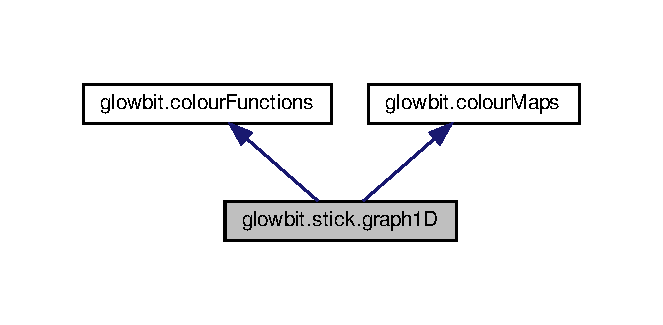
\includegraphics[width=318pt]{classglowbit_1_1stick_1_1graph1D__inherit__graph}
\end{center}
\end{figure}


Collaboration diagram for glowbit.\+stick.\+graph1D\+:\nopagebreak
\begin{figure}[H]
\begin{center}
\leavevmode
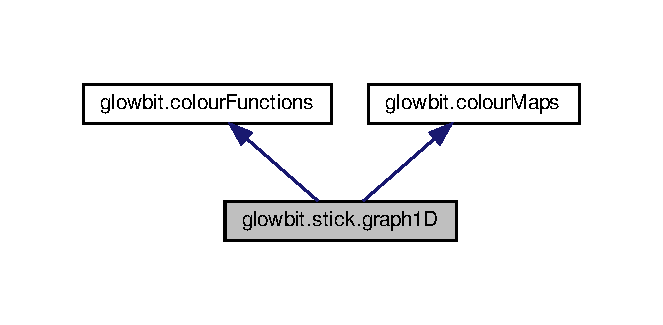
\includegraphics[width=318pt]{classglowbit_1_1stick_1_1graph1D__coll__graph}
\end{center}
\end{figure}
\subsection*{Public Member Functions}
\begin{DoxyCompactItemize}
\item 
\mbox{\Hypertarget{classglowbit_1_1stick_1_1graph1D_a46a0e6a76c186a975f7cc335faa9480f}\label{classglowbit_1_1stick_1_1graph1D_a46a0e6a76c186a975f7cc335faa9480f}} 
def {\bfseries \+\_\+\+\_\+init\+\_\+\+\_\+} (self, min\+Value=0, max\+Value=255, min\+Index=0, max\+Index=7, colour=0x\+F\+F\+F\+F\+F\+F, colour\+Map=\char`\"{}\+Solid\char`\"{}, update=\+False)
\end{DoxyCompactItemize}
\subsection*{Public Attributes}
\begin{DoxyCompactItemize}
\item 
\mbox{\Hypertarget{classglowbit_1_1stick_1_1graph1D_a1a0b5e32db369f6b6253a2010abd9927}\label{classglowbit_1_1stick_1_1graph1D_a1a0b5e32db369f6b6253a2010abd9927}} 
{\bfseries min\+Value}
\item 
\mbox{\Hypertarget{classglowbit_1_1stick_1_1graph1D_a3048e88f86ca331e54635ec2e6c60e5d}\label{classglowbit_1_1stick_1_1graph1D_a3048e88f86ca331e54635ec2e6c60e5d}} 
{\bfseries max\+Value}
\item 
\mbox{\Hypertarget{classglowbit_1_1stick_1_1graph1D_ad1e026360113687c6a2b6bec9f5b0cdc}\label{classglowbit_1_1stick_1_1graph1D_ad1e026360113687c6a2b6bec9f5b0cdc}} 
{\bfseries min\+Index}
\item 
\mbox{\Hypertarget{classglowbit_1_1stick_1_1graph1D_a76946ca7d21c9323bc75a7cb254178ff}\label{classglowbit_1_1stick_1_1graph1D_a76946ca7d21c9323bc75a7cb254178ff}} 
{\bfseries max\+Index}
\item 
\mbox{\Hypertarget{classglowbit_1_1stick_1_1graph1D_aa9e608ce7572fcd338d06431296c65ca}\label{classglowbit_1_1stick_1_1graph1D_aa9e608ce7572fcd338d06431296c65ca}} 
{\bfseries m}
\item 
\mbox{\Hypertarget{classglowbit_1_1stick_1_1graph1D_a5881c702849e31be5db908e316a18310}\label{classglowbit_1_1stick_1_1graph1D_a5881c702849e31be5db908e316a18310}} 
{\bfseries offset}
\item 
\mbox{\Hypertarget{classglowbit_1_1stick_1_1graph1D_aafaf7afb2c66c6b9c4edec4fc34c3722}\label{classglowbit_1_1stick_1_1graph1D_aafaf7afb2c66c6b9c4edec4fc34c3722}} 
{\bfseries update}
\item 
\mbox{\Hypertarget{classglowbit_1_1stick_1_1graph1D_aaad26d7930ec770e094d525c2cab12b8}\label{classglowbit_1_1stick_1_1graph1D_aaad26d7930ec770e094d525c2cab12b8}} 
{\bfseries colour}
\item 
\mbox{\Hypertarget{classglowbit_1_1stick_1_1graph1D_a52b7b7cc9d5385620272068f2255ddbd}\label{classglowbit_1_1stick_1_1graph1D_a52b7b7cc9d5385620272068f2255ddbd}} 
{\bfseries colour\+Map}
\end{DoxyCompactItemize}


The documentation for this class was generated from the following file\+:\begin{DoxyCompactItemize}
\item 
glowbit.\+py\end{DoxyCompactItemize}

\hypertarget{classglowbit_1_1glowbitMatrix_1_1graph2D}{}\section{glowbit.\+glowbit\+Matrix.\+graph2D Class Reference}
\label{classglowbit_1_1glowbitMatrix_1_1graph2D}\index{glowbit.\+glowbit\+Matrix.\+graph2D@{glowbit.\+glowbit\+Matrix.\+graph2D}}


Object for drawing 2 dimensional time series graphs on Glow\+Bit Matrix displays.  




Inheritance diagram for glowbit.\+glowbit\+Matrix.\+graph2D\+:\nopagebreak
\begin{figure}[H]
\begin{center}
\leavevmode
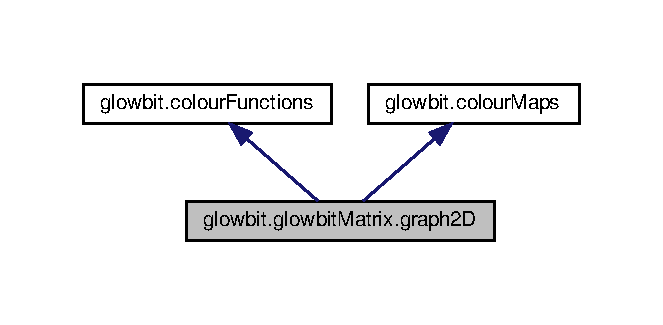
\includegraphics[width=318pt]{classglowbit_1_1glowbitMatrix_1_1graph2D__inherit__graph}
\end{center}
\end{figure}


Collaboration diagram for glowbit.\+glowbit\+Matrix.\+graph2D\+:\nopagebreak
\begin{figure}[H]
\begin{center}
\leavevmode
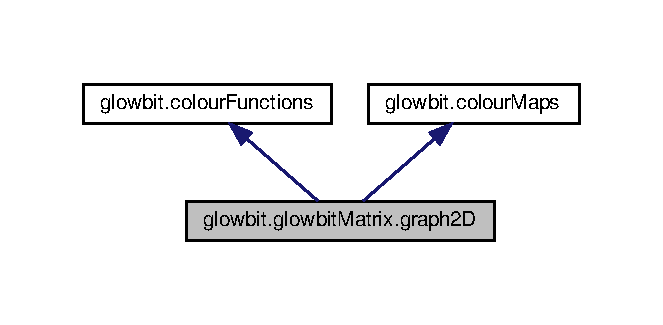
\includegraphics[width=318pt]{classglowbit_1_1glowbitMatrix_1_1graph2D__coll__graph}
\end{center}
\end{figure}
\subsection*{Public Member Functions}
\begin{DoxyCompactItemize}
\item 
def \hyperlink{classglowbit_1_1glowbitMatrix_1_1graph2D_a6250b96918df343764c1bc268a6e813b}{\+\_\+\+\_\+init\+\_\+\+\_\+} (self, originX=0, originY=7, width=8, height=8, min\+Value=0, max\+Value=255, colour=0x\+F\+F\+F\+F\+F\+F, bg\+Colour=0x000000, colour\+Map=\char`\"{}\+Solid\char`\"{}, update=\+False, bars=\+False)
\begin{DoxyCompactList}\small\item\em Initialisation routine for the glowbit.\+matrix.\+graph2D object. \end{DoxyCompactList}\end{DoxyCompactItemize}
\subsection*{Public Attributes}
\begin{DoxyCompactItemize}
\item 
\mbox{\Hypertarget{classglowbit_1_1glowbitMatrix_1_1graph2D_a6bd5d905ecb1687e4972d236242afd6c}\label{classglowbit_1_1glowbitMatrix_1_1graph2D_a6bd5d905ecb1687e4972d236242afd6c}} 
{\bfseries min\+Value}
\item 
\mbox{\Hypertarget{classglowbit_1_1glowbitMatrix_1_1graph2D_a1f8f137d2d109fd915658761911784fc}\label{classglowbit_1_1glowbitMatrix_1_1graph2D_a1f8f137d2d109fd915658761911784fc}} 
{\bfseries max\+Value}
\item 
\mbox{\Hypertarget{classglowbit_1_1glowbitMatrix_1_1graph2D_a49a68c7ea8a2bc525e28910525188dbb}\label{classglowbit_1_1glowbitMatrix_1_1graph2D_a49a68c7ea8a2bc525e28910525188dbb}} 
{\bfseries originX}
\item 
\mbox{\Hypertarget{classglowbit_1_1glowbitMatrix_1_1graph2D_a9ea2e93447b3a2da097e8a427bf69081}\label{classglowbit_1_1glowbitMatrix_1_1graph2D_a9ea2e93447b3a2da097e8a427bf69081}} 
{\bfseries originY}
\item 
\mbox{\Hypertarget{classglowbit_1_1glowbitMatrix_1_1graph2D_ada2b351af956e904bff60d74c4400b25}\label{classglowbit_1_1glowbitMatrix_1_1graph2D_ada2b351af956e904bff60d74c4400b25}} 
{\bfseries width}
\item 
\mbox{\Hypertarget{classglowbit_1_1glowbitMatrix_1_1graph2D_ab201ddb2948cb34c03f7c69824a89d3a}\label{classglowbit_1_1glowbitMatrix_1_1graph2D_ab201ddb2948cb34c03f7c69824a89d3a}} 
{\bfseries height}
\item 
\mbox{\Hypertarget{classglowbit_1_1glowbitMatrix_1_1graph2D_aed92b1ababdf74d8f76b24e162a1cdc1}\label{classglowbit_1_1glowbitMatrix_1_1graph2D_aed92b1ababdf74d8f76b24e162a1cdc1}} 
{\bfseries colour}
\item 
\mbox{\Hypertarget{classglowbit_1_1glowbitMatrix_1_1graph2D_ad832ef76bb6603f4ecac44964cad3a2f}\label{classglowbit_1_1glowbitMatrix_1_1graph2D_ad832ef76bb6603f4ecac44964cad3a2f}} 
{\bfseries bg\+Colour}
\item 
\mbox{\Hypertarget{classglowbit_1_1glowbitMatrix_1_1graph2D_a623c46f1b3d650613489dbcf407a0061}\label{classglowbit_1_1glowbitMatrix_1_1graph2D_a623c46f1b3d650613489dbcf407a0061}} 
{\bfseries update}
\item 
\mbox{\Hypertarget{classglowbit_1_1glowbitMatrix_1_1graph2D_a66f64dbba8f077506ad52165f4c3d9e3}\label{classglowbit_1_1glowbitMatrix_1_1graph2D_a66f64dbba8f077506ad52165f4c3d9e3}} 
{\bfseries m}
\item 
\mbox{\Hypertarget{classglowbit_1_1glowbitMatrix_1_1graph2D_ac8cfe4f990570e96ee4afd5d9400371b}\label{classglowbit_1_1glowbitMatrix_1_1graph2D_ac8cfe4f990570e96ee4afd5d9400371b}} 
{\bfseries offset}
\item 
\mbox{\Hypertarget{classglowbit_1_1glowbitMatrix_1_1graph2D_a3dc420308e355151a6e6d1943a473a94}\label{classglowbit_1_1glowbitMatrix_1_1graph2D_a3dc420308e355151a6e6d1943a473a94}} 
{\bfseries bars}
\item 
\mbox{\Hypertarget{classglowbit_1_1glowbitMatrix_1_1graph2D_a5a11fc642d5ad79ab08e5d806b0bab77}\label{classglowbit_1_1glowbitMatrix_1_1graph2D_a5a11fc642d5ad79ab08e5d806b0bab77}} 
{\bfseries data}
\item 
\mbox{\Hypertarget{classglowbit_1_1glowbitMatrix_1_1graph2D_a116e7d95ab5e0b13ea8f57582bfa15e4}\label{classglowbit_1_1glowbitMatrix_1_1graph2D_a116e7d95ab5e0b13ea8f57582bfa15e4}} 
{\bfseries colour\+Map}
\end{DoxyCompactItemize}


\subsection{Detailed Description}
Object for drawing 2 dimensional time series graphs on Glow\+Bit Matrix displays. 



\subsection{Constructor \& Destructor Documentation}
\mbox{\Hypertarget{classglowbit_1_1glowbitMatrix_1_1graph2D_a6250b96918df343764c1bc268a6e813b}\label{classglowbit_1_1glowbitMatrix_1_1graph2D_a6250b96918df343764c1bc268a6e813b}} 
\index{glowbit\+::glowbit\+Matrix\+::graph2D@{glowbit\+::glowbit\+Matrix\+::graph2D}!\+\_\+\+\_\+init\+\_\+\+\_\+@{\+\_\+\+\_\+init\+\_\+\+\_\+}}
\index{\+\_\+\+\_\+init\+\_\+\+\_\+@{\+\_\+\+\_\+init\+\_\+\+\_\+}!glowbit\+::glowbit\+Matrix\+::graph2D@{glowbit\+::glowbit\+Matrix\+::graph2D}}
\subsubsection{\texorpdfstring{\+\_\+\+\_\+init\+\_\+\+\_\+()}{\_\_init\_\_()}}
{\footnotesize\ttfamily def glowbit.\+glowbit\+Matrix.\+graph2\+D.\+\_\+\+\_\+init\+\_\+\+\_\+ (\begin{DoxyParamCaption}\item[{}]{self,  }\item[{}]{originX = {\ttfamily 0},  }\item[{}]{originY = {\ttfamily 7},  }\item[{}]{width = {\ttfamily 8},  }\item[{}]{height = {\ttfamily 8},  }\item[{}]{min\+Value = {\ttfamily 0},  }\item[{}]{max\+Value = {\ttfamily 255},  }\item[{}]{colour = {\ttfamily 0xFFFFFF},  }\item[{}]{bg\+Colour = {\ttfamily 0x000000},  }\item[{}]{colour\+Map = {\ttfamily \char`\"{}Solid\char`\"{}},  }\item[{}]{update = {\ttfamily False},  }\item[{}]{bars = {\ttfamily False} }\end{DoxyParamCaption})}



Initialisation routine for the glowbit.\+matrix.\+graph2D object. 

A \hyperlink{classglowbit_1_1glowbitMatrix_1_1graph2D}{graph2D} object will be drawn to a rectangular region specified by the origin, width, and height.

This graph type is explicitly designed to draw time series data.


\begin{DoxyParams}{Parameters}
{\em originX} & The x coordinate of the graph\textquotesingle{}s origin (lower left corner). \\
\hline
{\em originY} & The y coordinate of the graph\textquotesingle{}s origin (lower left corner). \\
\hline
{\em width} & The width, in pixels, of the graph\textquotesingle{}s drawing area. \\
\hline
{\em height} & The height, in pixels, of the graph\textquotesingle{}s drawing area \\
\hline
{\em min\+Value} & The value which will be mapped to the bottom edge. \\
\hline
{\em max\+Value} & The value which will be mapped to the upper edge. \\
\hline
{\em colour} & A packed 32-\/bit Glow\+Bit colour value. Used by the \char`\"{}\+Solid\char`\"{} colourmap, ignored by the \char`\"{}\+Rainbow\char`\"{} colourmap. Can also be accessed when writing custom colour map functions. \\
\hline
{\em bg\+Colour} & A packed 32-\/bit Glow\+Bit colour value which is drawn to the entire graph area prior to drawing the data. \\
\hline
{\em colour\+Map} & Either the string \char`\"{}\+Solid\char`\"{} or \char`\"{}\+Rainbow\char`\"{} or a pointer to a custom colour map function. Custom colour maps must take the parameters colour\+Map(self, index, min\+Index, max\+Index). \\
\hline
{\em update} & If update=True then a call to \hyperlink{classglowbit_1_1glowbitMatrix_ae9083babec0d5004363782540b60baed}{update\+Graph2\+D()} will, in turn, call \hyperlink{classglowbit_1_1glowbit_a051aed2a4969fdcb0466e4e840209279}{glowbit.\+pixels\+Show()} to update the physical L\+E\+Ds. \\
\hline
\end{DoxyParams}


The documentation for this class was generated from the following file\+:\begin{DoxyCompactItemize}
\item 
glowbit.\+py\end{DoxyCompactItemize}

\hypertarget{classglowbit_1_1matrix4x4}{}\section{glowbit.\+matrix4x4 Class Reference}
\label{classglowbit_1_1matrix4x4}\index{glowbit.\+matrix4x4@{glowbit.\+matrix4x4}}


Inheritance diagram for glowbit.\+matrix4x4\+:\nopagebreak
\begin{figure}[H]
\begin{center}
\leavevmode
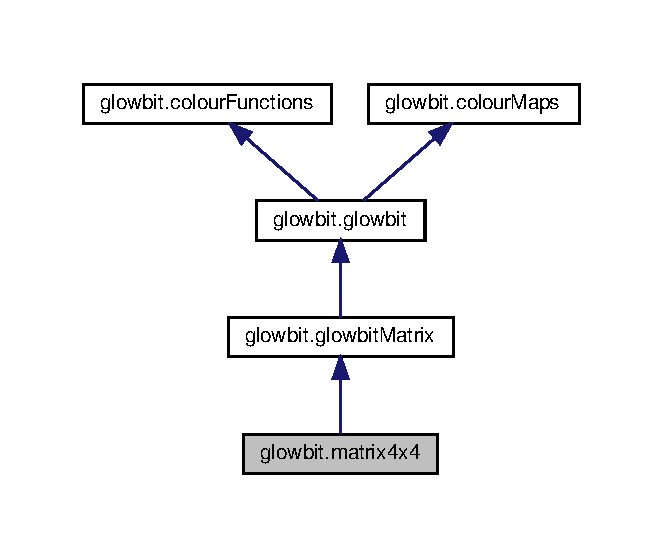
\includegraphics[width=199pt]{classglowbit_1_1matrix4x4__inherit__graph}
\end{center}
\end{figure}


Collaboration diagram for glowbit.\+matrix4x4\+:\nopagebreak
\begin{figure}[H]
\begin{center}
\leavevmode
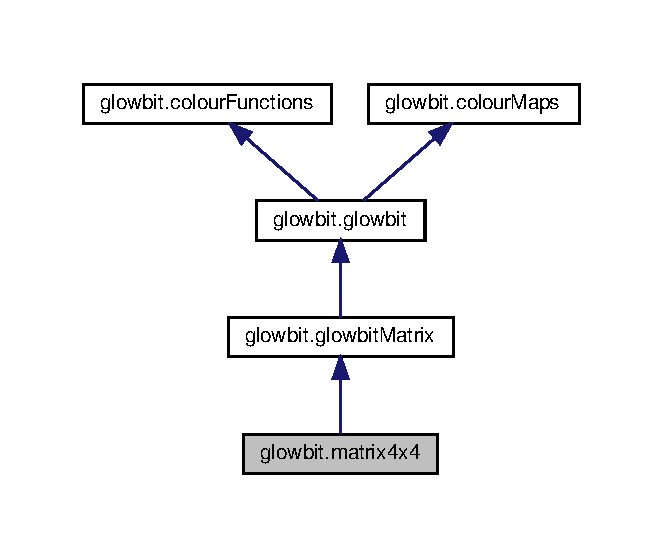
\includegraphics[width=199pt]{classglowbit_1_1matrix4x4__coll__graph}
\end{center}
\end{figure}
\subsection*{Public Member Functions}
\begin{DoxyCompactItemize}
\item 
\mbox{\Hypertarget{classglowbit_1_1matrix4x4_a9a9f870a9505b2a4e27519a8e279e81c}\label{classglowbit_1_1matrix4x4_a9a9f870a9505b2a4e27519a8e279e81c}} 
def {\bfseries \+\_\+\+\_\+init\+\_\+\+\_\+} (self, tiles=1, pin=18, brightness=20, map\+Function=None, rate\+Limit\+F\+PS=30, sm=0)
\item 
\mbox{\Hypertarget{classglowbit_1_1matrix4x4_aea814e3be265990137d4027ae181e58d}\label{classglowbit_1_1matrix4x4_aea814e3be265990137d4027ae181e58d}} 
def {\bfseries remap4x4} (self, x, y)
\end{DoxyCompactItemize}
\subsection*{Public Attributes}
\begin{DoxyCompactItemize}
\item 
\mbox{\Hypertarget{classglowbit_1_1matrix4x4_ac8fda7286a04f0b1ee41410b2dbdfdd5}\label{classglowbit_1_1matrix4x4_ac8fda7286a04f0b1ee41410b2dbdfdd5}} 
{\bfseries sm}
\item 
\mbox{\Hypertarget{classglowbit_1_1matrix4x4_a993d1806e4f7a90441ebdf1220edb1a7}\label{classglowbit_1_1matrix4x4_a993d1806e4f7a90441ebdf1220edb1a7}} 
{\bfseries pixels\+Show}
\item 
\mbox{\Hypertarget{classglowbit_1_1matrix4x4_ab9f1182e7170613d05eda41961882e07}\label{classglowbit_1_1matrix4x4_ab9f1182e7170613d05eda41961882e07}} 
{\bfseries ticks\+\_\+ms}
\item 
\mbox{\Hypertarget{classglowbit_1_1matrix4x4_a3c259adf79688e61a5a9034adfa54fe2}\label{classglowbit_1_1matrix4x4_a3c259adf79688e61a5a9034adfa54fe2}} 
{\bfseries tiles}
\item 
\mbox{\Hypertarget{classglowbit_1_1matrix4x4_a4f4aaad1bb8a7707e2e77194813f3fa9}\label{classglowbit_1_1matrix4x4_a4f4aaad1bb8a7707e2e77194813f3fa9}} 
{\bfseries num\+L\+E\+Ds}
\item 
\mbox{\Hypertarget{classglowbit_1_1matrix4x4_add268b0983abd2dd623efc8762eb46a6}\label{classglowbit_1_1matrix4x4_add268b0983abd2dd623efc8762eb46a6}} 
{\bfseries num\+L\+E\+DsX}
\item 
\mbox{\Hypertarget{classglowbit_1_1matrix4x4_a6fb20d31028c50c2eac76ba028f265f7}\label{classglowbit_1_1matrix4x4_a6fb20d31028c50c2eac76ba028f265f7}} 
{\bfseries num\+L\+E\+DsY}
\item 
\mbox{\Hypertarget{classglowbit_1_1matrix4x4_a27b1e9f3a7c4b5614663d76cb6f7b9cc}\label{classglowbit_1_1matrix4x4_a27b1e9f3a7c4b5614663d76cb6f7b9cc}} 
{\bfseries strip}
\item 
\mbox{\Hypertarget{classglowbit_1_1matrix4x4_a6c004d9d95fca084c71dd549d8f02418}\label{classglowbit_1_1matrix4x4_a6c004d9d95fca084c71dd549d8f02418}} 
{\bfseries ar}
\item 
\mbox{\Hypertarget{classglowbit_1_1matrix4x4_a1adfc56eb47b5bfc5d3102efaeb38097}\label{classglowbit_1_1matrix4x4_a1adfc56eb47b5bfc5d3102efaeb38097}} 
{\bfseries dimmer\+\_\+ar}
\item 
\mbox{\Hypertarget{classglowbit_1_1matrix4x4_afc755575c2642804d5c6eac170723064}\label{classglowbit_1_1matrix4x4_afc755575c2642804d5c6eac170723064}} 
{\bfseries last\+Frame\+\_\+ms}
\item 
\mbox{\Hypertarget{classglowbit_1_1matrix4x4_a60001cda5a86c8d035838f528e3428dc}\label{classglowbit_1_1matrix4x4_a60001cda5a86c8d035838f528e3428dc}} 
{\bfseries scrolling\+Text}
\item 
\mbox{\Hypertarget{classglowbit_1_1matrix4x4_aaa175c98bbdcb35a83dd59192ee0686f}\label{classglowbit_1_1matrix4x4_aaa175c98bbdcb35a83dd59192ee0686f}} 
{\bfseries brightness}
\item 
\mbox{\Hypertarget{classglowbit_1_1matrix4x4_a8d2971111428adb5e6ed35b6f07b63de}\label{classglowbit_1_1matrix4x4_a8d2971111428adb5e6ed35b6f07b63de}} 
{\bfseries remap}
\item 
\mbox{\Hypertarget{classglowbit_1_1matrix4x4_acfc0f73dcf2d58bb48aec88b6fc0eb33}\label{classglowbit_1_1matrix4x4_acfc0f73dcf2d58bb48aec88b6fc0eb33}} 
{\bfseries rate\+Limit}
\end{DoxyCompactItemize}
\subsection*{Additional Inherited Members}


The documentation for this class was generated from the following file\+:\begin{DoxyCompactItemize}
\item 
glowbit.\+py\end{DoxyCompactItemize}

\hypertarget{classglowbit_1_1matrix8x8}{}\section{glowbit.\+matrix8x8 Class Reference}
\label{classglowbit_1_1matrix8x8}\index{glowbit.\+matrix8x8@{glowbit.\+matrix8x8}}


Inheritance diagram for glowbit.\+matrix8x8\+:\nopagebreak
\begin{figure}[H]
\begin{center}
\leavevmode
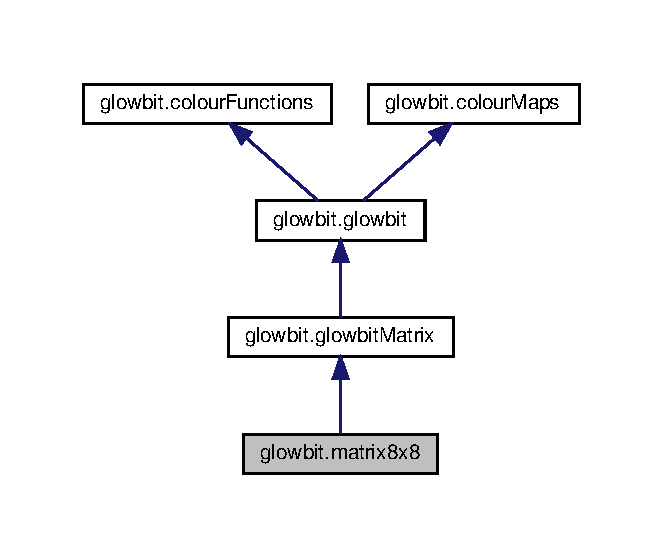
\includegraphics[width=199pt]{classglowbit_1_1matrix8x8__inherit__graph}
\end{center}
\end{figure}


Collaboration diagram for glowbit.\+matrix8x8\+:\nopagebreak
\begin{figure}[H]
\begin{center}
\leavevmode
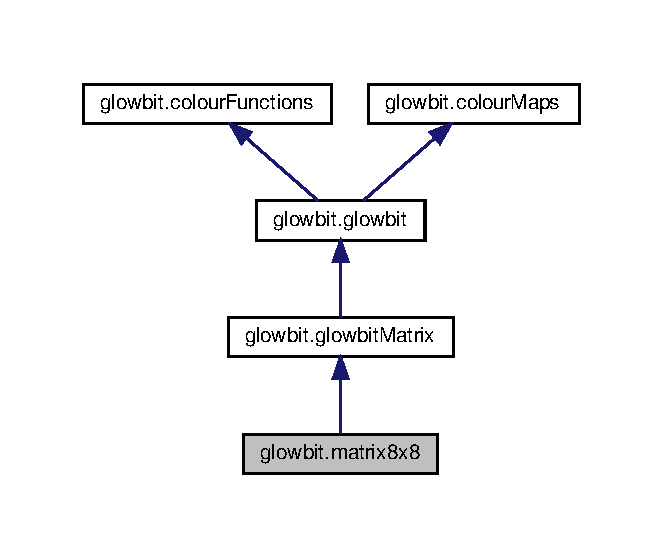
\includegraphics[width=199pt]{classglowbit_1_1matrix8x8__coll__graph}
\end{center}
\end{figure}
\subsection*{Classes}
\begin{DoxyCompactItemize}
\item 
class \hyperlink{classglowbit_1_1matrix8x8_1_1textScroll}{text\+Scroll}
\end{DoxyCompactItemize}
\subsection*{Public Member Functions}
\begin{DoxyCompactItemize}
\item 
\mbox{\Hypertarget{classglowbit_1_1matrix8x8_a7b30f3aec73c8a938a063ea640899af6}\label{classglowbit_1_1matrix8x8_a7b30f3aec73c8a938a063ea640899af6}} 
def {\bfseries \+\_\+\+\_\+init\+\_\+\+\_\+} (self, tile\+Rows=1, tile\+Cols=1, pin=18, brightness=20, map\+Function=None, rate\+Limit\+F\+PS=-\/1, rate\+Limit\+Characters\+Per\+Second=-\/1, sm=0)
\item 
\mbox{\Hypertarget{classglowbit_1_1matrix8x8_a1db0574d73977d46ba90068b9970777f}\label{classglowbit_1_1matrix8x8_a1db0574d73977d46ba90068b9970777f}} 
def {\bfseries print\+Text\+Wrap} (self, string, x=0, y=0, colour=0x\+F\+F\+F\+F\+F\+F)
\item 
\mbox{\Hypertarget{classglowbit_1_1matrix8x8_ade5b8578e6c38d86f356cdb6997cc314}\label{classglowbit_1_1matrix8x8_ade5b8578e6c38d86f356cdb6997cc314}} 
def {\bfseries add\+Text\+Scroll} (self, string, y=0, x=0, colour=0x\+F\+F\+F\+F\+F\+F, bg\+Colour=0x000000, update=\+False, blocking=\+False)
\item 
\mbox{\Hypertarget{classglowbit_1_1matrix8x8_a4a529f9b42ea95cc0f5dafcb0085d096}\label{classglowbit_1_1matrix8x8_a4a529f9b42ea95cc0f5dafcb0085d096}} 
def {\bfseries update\+Text\+Scroll} (self)
\item 
\mbox{\Hypertarget{classglowbit_1_1matrix8x8_a67146ad236571bf9e87fe7a847c8a1d1}\label{classglowbit_1_1matrix8x8_a67146ad236571bf9e87fe7a847c8a1d1}} 
def {\bfseries remap8x8} (self, x, y)
\item 
\mbox{\Hypertarget{classglowbit_1_1matrix8x8_a4ba16a1fa6231654833d619f8789275a}\label{classglowbit_1_1matrix8x8_a4ba16a1fa6231654833d619f8789275a}} 
def {\bfseries draw\+Char} (self, char, Px, Py, colour)
\item 
def \hyperlink{classglowbit_1_1matrix8x8_a5dfbe10ccf2acca4d6d4012e29e7b439}{update\+Rate\+Limit\+Characters\+Per\+Second} (self, rate\+Limit\+Characters\+Per\+Second)
\begin{DoxyCompactList}\small\item\em Changes the 8x8 matrix display\textquotesingle{}s update rate in units of \char`\"{}characters of scrolling text per second\char`\"{}. \end{DoxyCompactList}\end{DoxyCompactItemize}
\subsection*{Public Attributes}
\begin{DoxyCompactItemize}
\item 
\mbox{\Hypertarget{classglowbit_1_1matrix8x8_a739f238cd08f8d1baee326e1b39f8c6c}\label{classglowbit_1_1matrix8x8_a739f238cd08f8d1baee326e1b39f8c6c}} 
{\bfseries tile\+Rows}
\item 
\mbox{\Hypertarget{classglowbit_1_1matrix8x8_ad3c6a50f6b460b132773cea052fff106}\label{classglowbit_1_1matrix8x8_ad3c6a50f6b460b132773cea052fff106}} 
{\bfseries tile\+Cols}
\item 
\mbox{\Hypertarget{classglowbit_1_1matrix8x8_a9b656c42c8fda29877836bc4fbced6fa}\label{classglowbit_1_1matrix8x8_a9b656c42c8fda29877836bc4fbced6fa}} 
{\bfseries num\+L\+E\+Ds}
\item 
\mbox{\Hypertarget{classglowbit_1_1matrix8x8_a957c49a14c90493b5cb5cfe7c4dbd203}\label{classglowbit_1_1matrix8x8_a957c49a14c90493b5cb5cfe7c4dbd203}} 
{\bfseries num\+L\+E\+DsX}
\item 
\mbox{\Hypertarget{classglowbit_1_1matrix8x8_ab9abe55b6cce8cbce7e29d307a555d0a}\label{classglowbit_1_1matrix8x8_ab9abe55b6cce8cbce7e29d307a555d0a}} 
{\bfseries num\+L\+E\+DsY}
\item 
\mbox{\Hypertarget{classglowbit_1_1matrix8x8_a9148a02f6c6d48d1745ec9b801d58083}\label{classglowbit_1_1matrix8x8_a9148a02f6c6d48d1745ec9b801d58083}} 
{\bfseries sm}
\item 
\mbox{\Hypertarget{classglowbit_1_1matrix8x8_aa0c38c2d52806ba5c9d2ffbc7734b364}\label{classglowbit_1_1matrix8x8_aa0c38c2d52806ba5c9d2ffbc7734b364}} 
{\bfseries pixels\+Show}
\item 
\mbox{\Hypertarget{classglowbit_1_1matrix8x8_a83010a4dfcef0755c55950a1703e7e13}\label{classglowbit_1_1matrix8x8_a83010a4dfcef0755c55950a1703e7e13}} 
{\bfseries ticks\+\_\+ms}
\item 
\mbox{\Hypertarget{classglowbit_1_1matrix8x8_ac29e07887369c313893b4ca71f3f86c3}\label{classglowbit_1_1matrix8x8_ac29e07887369c313893b4ca71f3f86c3}} 
{\bfseries strip}
\item 
\mbox{\Hypertarget{classglowbit_1_1matrix8x8_af41df10fb7fe285edcf2a7a4677854cc}\label{classglowbit_1_1matrix8x8_af41df10fb7fe285edcf2a7a4677854cc}} 
{\bfseries ar}
\item 
\mbox{\Hypertarget{classglowbit_1_1matrix8x8_a018d52a73e4f3902ca3272ae1e6f552c}\label{classglowbit_1_1matrix8x8_a018d52a73e4f3902ca3272ae1e6f552c}} 
{\bfseries dimmer\+\_\+ar}
\item 
\mbox{\Hypertarget{classglowbit_1_1matrix8x8_a4d227ae72c97ff008677711fc3274104}\label{classglowbit_1_1matrix8x8_a4d227ae72c97ff008677711fc3274104}} 
{\bfseries brightness}
\item 
\mbox{\Hypertarget{classglowbit_1_1matrix8x8_abaee6a53b3a15537cb75133abc6edb22}\label{classglowbit_1_1matrix8x8_abaee6a53b3a15537cb75133abc6edb22}} 
{\bfseries scrolling\+Text}
\item 
\mbox{\Hypertarget{classglowbit_1_1matrix8x8_a9f9e4c792c4420744234f8c400f1dc54}\label{classglowbit_1_1matrix8x8_a9f9e4c792c4420744234f8c400f1dc54}} 
{\bfseries last\+Frame\+\_\+ms}
\item 
\mbox{\Hypertarget{classglowbit_1_1matrix8x8_a04e1bdcc67b521246610c68f5dafaa3e}\label{classglowbit_1_1matrix8x8_a04e1bdcc67b521246610c68f5dafaa3e}} 
{\bfseries rate\+Limit}
\item 
\mbox{\Hypertarget{classglowbit_1_1matrix8x8_af0afcefd1ec2dc8614e5f8f7478fd36c}\label{classglowbit_1_1matrix8x8_af0afcefd1ec2dc8614e5f8f7478fd36c}} 
{\bfseries scrolling\+Text\+List}
\item 
\mbox{\Hypertarget{classglowbit_1_1matrix8x8_a458b71109effe56dcbb6cde442cf5657}\label{classglowbit_1_1matrix8x8_a458b71109effe56dcbb6cde442cf5657}} 
{\bfseries remap}
\item 
\mbox{\Hypertarget{classglowbit_1_1matrix8x8_aad3eb346cc87f36b36eb8bc6aeb67e5f}\label{classglowbit_1_1matrix8x8_aad3eb346cc87f36b36eb8bc6aeb67e5f}} 
{\bfseries update\+Text}
\item 
\mbox{\Hypertarget{classglowbit_1_1matrix8x8_af983fb390e954e9b45f0c1ce11ffbe56}\label{classglowbit_1_1matrix8x8_af983fb390e954e9b45f0c1ce11ffbe56}} 
{\bfseries update}
\end{DoxyCompactItemize}
\subsection*{Additional Inherited Members}


\subsection{Member Function Documentation}
\mbox{\Hypertarget{classglowbit_1_1matrix8x8_a5dfbe10ccf2acca4d6d4012e29e7b439}\label{classglowbit_1_1matrix8x8_a5dfbe10ccf2acca4d6d4012e29e7b439}} 
\index{glowbit\+::matrix8x8@{glowbit\+::matrix8x8}!update\+Rate\+Limit\+Characters\+Per\+Second@{update\+Rate\+Limit\+Characters\+Per\+Second}}
\index{update\+Rate\+Limit\+Characters\+Per\+Second@{update\+Rate\+Limit\+Characters\+Per\+Second}!glowbit\+::matrix8x8@{glowbit\+::matrix8x8}}
\subsubsection{\texorpdfstring{update\+Rate\+Limit\+Characters\+Per\+Second()}{updateRateLimitCharactersPerSecond()}}
{\footnotesize\ttfamily def glowbit.\+matrix8x8.\+update\+Rate\+Limit\+Characters\+Per\+Second (\begin{DoxyParamCaption}\item[{}]{self,  }\item[{}]{rate\+Limit\+Characters\+Per\+Second }\end{DoxyParamCaption})}



Changes the 8x8 matrix display\textquotesingle{}s update rate in units of \char`\"{}characters of scrolling text per second\char`\"{}. 

For example, a value of 2 would scroll 2 charcters per second; leaving each character at least partly visible for 0.\+5 seconds. 

The documentation for this class was generated from the following file\+:\begin{DoxyCompactItemize}
\item 
glowbit.\+py\end{DoxyCompactItemize}

\hypertarget{classglowbit_1_1micropython}{}\section{glowbit.\+micropython Class Reference}
\label{classglowbit_1_1micropython}\index{glowbit.\+micropython@{glowbit.\+micropython}}
\subsection*{Public Member Functions}
\begin{DoxyCompactItemize}
\item 
\mbox{\Hypertarget{classglowbit_1_1micropython_a37370a837bfad970b380b72a9071b1b5}\label{classglowbit_1_1micropython_a37370a837bfad970b380b72a9071b1b5}} 
def {\bfseries viper} (func)
\end{DoxyCompactItemize}


The documentation for this class was generated from the following file\+:\begin{DoxyCompactItemize}
\item 
glowbit.\+py\end{DoxyCompactItemize}

\hypertarget{classglowbit_1_1rp2_1_1PIO}{}\section{glowbit.\+rp2.\+P\+IO Class Reference}
\label{classglowbit_1_1rp2_1_1PIO}\index{glowbit.\+rp2.\+P\+IO@{glowbit.\+rp2.\+P\+IO}}
\subsection*{Static Public Attributes}
\begin{DoxyCompactItemize}
\item 
\mbox{\Hypertarget{classglowbit_1_1rp2_1_1PIO_a5621c6b4c70eb35dc4beacf13451c826}\label{classglowbit_1_1rp2_1_1PIO_a5621c6b4c70eb35dc4beacf13451c826}} 
{\bfseries O\+U\+T\+\_\+\+L\+OW} = None
\item 
\mbox{\Hypertarget{classglowbit_1_1rp2_1_1PIO_a945bdbedbb97c7d792c568df1ca2b2d6}\label{classglowbit_1_1rp2_1_1PIO_a945bdbedbb97c7d792c568df1ca2b2d6}} 
{\bfseries S\+H\+I\+F\+T\+\_\+\+L\+E\+FT} = None
\end{DoxyCompactItemize}


The documentation for this class was generated from the following file\+:\begin{DoxyCompactItemize}
\item 
glowbit.\+py\end{DoxyCompactItemize}

\hypertarget{classglowbit_1_1stick_1_1pulse}{}\section{glowbit.\+stick.\+pulse Class Reference}
\label{classglowbit_1_1stick_1_1pulse}\index{glowbit.\+stick.\+pulse@{glowbit.\+stick.\+pulse}}


A class for animating \char`\"{}pulses\char`\"{} which move down a Glow\+Bit stick.  




Inheritance diagram for glowbit.\+stick.\+pulse\+:\nopagebreak
\begin{figure}[H]
\begin{center}
\leavevmode
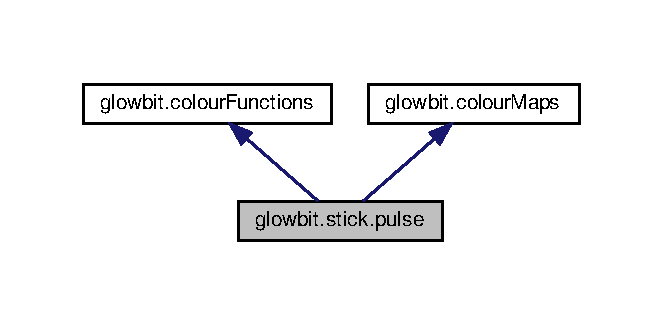
\includegraphics[width=318pt]{classglowbit_1_1stick_1_1pulse__inherit__graph}
\end{center}
\end{figure}


Collaboration diagram for glowbit.\+stick.\+pulse\+:\nopagebreak
\begin{figure}[H]
\begin{center}
\leavevmode
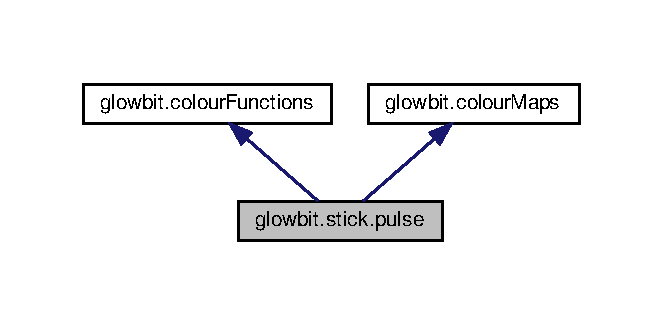
\includegraphics[width=318pt]{classglowbit_1_1stick_1_1pulse__coll__graph}
\end{center}
\end{figure}
\subsection*{Public Member Functions}
\begin{DoxyCompactItemize}
\item 
def \hyperlink{classglowbit_1_1stick_1_1pulse_a53a1dbcea6d84002f76f9c10c7ae0481}{\+\_\+\+\_\+init\+\_\+\+\_\+} (self, \hyperlink{classglowbit_1_1stick_1_1pulse_ac600e5460c9f05e36ea6d7b7cef0c763}{speed}=100, \hyperlink{classglowbit_1_1stick_1_1pulse_a1b0b4b29bc1a9bbd90d9f919589a560a}{colour}=\mbox{[}0x\+F\+F\+F\+F\+F\+F\mbox{]}, index=0, colour\+Map=\+None)
\begin{DoxyCompactList}\small\item\em Initialisation routine for the Glow\+Bit Stick pulse object. \end{DoxyCompactList}\end{DoxyCompactItemize}
\subsection*{Public Attributes}
\begin{DoxyCompactItemize}
\item 
\mbox{\Hypertarget{classglowbit_1_1stick_1_1pulse_ac600e5460c9f05e36ea6d7b7cef0c763}\label{classglowbit_1_1stick_1_1pulse_ac600e5460c9f05e36ea6d7b7cef0c763}} 
\hyperlink{classglowbit_1_1stick_1_1pulse_ac600e5460c9f05e36ea6d7b7cef0c763}{speed}
\begin{DoxyCompactList}\small\item\em Speed of the pulse. \end{DoxyCompactList}\item 
\mbox{\Hypertarget{classglowbit_1_1stick_1_1pulse_a7b5b6ddb2b400a838fbd8ec7819a4639}\label{classglowbit_1_1stick_1_1pulse_a7b5b6ddb2b400a838fbd8ec7819a4639}} 
\hyperlink{classglowbit_1_1stick_1_1pulse_a7b5b6ddb2b400a838fbd8ec7819a4639}{index}
\begin{DoxyCompactList}\small\item\em Initial index of the pulse. \end{DoxyCompactList}\item 
\hyperlink{classglowbit_1_1stick_1_1pulse_a1b0b4b29bc1a9bbd90d9f919589a560a}{colour}
\begin{DoxyCompactList}\small\item\em A list of 32-\/bit Glow\+Bit colour values. \end{DoxyCompactList}\item 
\hyperlink{classglowbit_1_1stick_1_1pulse_a11a715a74934bb938e8e826da29aac67}{colour\+Map}
\begin{DoxyCompactList}\small\item\em Either the string \char`\"{}\+Solid\char`\"{} or \char`\"{}\+Rainbow\char`\"{} or a function pointer to a custom colourmap. \end{DoxyCompactList}\end{DoxyCompactItemize}


\subsection{Detailed Description}
A class for animating \char`\"{}pulses\char`\"{} which move down a Glow\+Bit stick. 



\subsection{Constructor \& Destructor Documentation}
\mbox{\Hypertarget{classglowbit_1_1stick_1_1pulse_a53a1dbcea6d84002f76f9c10c7ae0481}\label{classglowbit_1_1stick_1_1pulse_a53a1dbcea6d84002f76f9c10c7ae0481}} 
\index{glowbit\+::stick\+::pulse@{glowbit\+::stick\+::pulse}!\+\_\+\+\_\+init\+\_\+\+\_\+@{\+\_\+\+\_\+init\+\_\+\+\_\+}}
\index{\+\_\+\+\_\+init\+\_\+\+\_\+@{\+\_\+\+\_\+init\+\_\+\+\_\+}!glowbit\+::stick\+::pulse@{glowbit\+::stick\+::pulse}}
\subsubsection{\texorpdfstring{\+\_\+\+\_\+init\+\_\+\+\_\+()}{\_\_init\_\_()}}
{\footnotesize\ttfamily def glowbit.\+stick.\+pulse.\+\_\+\+\_\+init\+\_\+\+\_\+ (\begin{DoxyParamCaption}\item[{}]{self,  }\item[{}]{speed = {\ttfamily 100},  }\item[{}]{colour = {\ttfamily \mbox{[}0xFFFFFF\mbox{]}},  }\item[{}]{index = {\ttfamily 0},  }\item[{}]{colour\+Map = {\ttfamily None} }\end{DoxyParamCaption})}



Initialisation routine for the Glow\+Bit Stick pulse object. 

This function uses the \hyperlink{classglowbit_1_1glowbit_a0db675789faef3399ffb2c1213c12048}{pixel\+Saturating\+Add()} method so multiple pulses can be drawn without colour values corrupting due to addition overflow.


\begin{DoxyParams}{Parameters}
{\em speed} & The speed of the pulse in units of (pixels moved per frame) $\ast$ 100. A value of 100 means the pulse will move 1 pixels per frame. A speed of 1 will move a pulse 1 pixel every 100 frames. Speed can be positive or negative to allow pulses to move in either direction. \\
\hline
{\em colour} & A list of 32-\/bit Glow\+Bit colours for the pulse. The pulse will have a width equal to the number of elements in this list. A list entry of -\/1 will have the colour set by a colour map function. \\
\hline
{\em index} & The initial index of the pulse. Generally recommended to set to 0 if speed $>$ 0 and num\+L\+E\+Ds if speed $<$ 0. \\
\hline
{\em colour\+Map} & Either the string \char`\"{}\+Solid\char`\"{} or \char`\"{}\+Rainbow\char`\"{} or a custom function pointer. Custom functions must take the positional arguments\+: colour\+Map\+Function(self, index, min\+Index, max\+Index). When calling colour map functions \hyperlink{classglowbit_1_1stick_a84e72d81b9c96b1acb268b730866a8ea}{update\+Pulses()} sets min\+Index to 0 and max\+Index to num\+L\+E\+Ds. \\
\hline
\end{DoxyParams}


\subsection{Member Data Documentation}
\mbox{\Hypertarget{classglowbit_1_1stick_1_1pulse_a1b0b4b29bc1a9bbd90d9f919589a560a}\label{classglowbit_1_1stick_1_1pulse_a1b0b4b29bc1a9bbd90d9f919589a560a}} 
\index{glowbit\+::stick\+::pulse@{glowbit\+::stick\+::pulse}!colour@{colour}}
\index{colour@{colour}!glowbit\+::stick\+::pulse@{glowbit\+::stick\+::pulse}}
\subsubsection{\texorpdfstring{colour}{colour}}
{\footnotesize\ttfamily glowbit.\+stick.\+pulse.\+colour}



A list of 32-\/bit Glow\+Bit colour values. 

Each one is drawn to a pixel; a -\/1 indicates the use of the colour\+Map function \mbox{\Hypertarget{classglowbit_1_1stick_1_1pulse_a11a715a74934bb938e8e826da29aac67}\label{classglowbit_1_1stick_1_1pulse_a11a715a74934bb938e8e826da29aac67}} 
\index{glowbit\+::stick\+::pulse@{glowbit\+::stick\+::pulse}!colour\+Map@{colour\+Map}}
\index{colour\+Map@{colour\+Map}!glowbit\+::stick\+::pulse@{glowbit\+::stick\+::pulse}}
\subsubsection{\texorpdfstring{colour\+Map}{colourMap}}
{\footnotesize\ttfamily glowbit.\+stick.\+pulse.\+colour\+Map}



Either the string \char`\"{}\+Solid\char`\"{} or \char`\"{}\+Rainbow\char`\"{} or a function pointer to a custom colourmap. 

Only sets pixel colour for pixels with a colour of -\/1. 

The documentation for this class was generated from the following file\+:\begin{DoxyCompactItemize}
\item 
glowbit.\+py\end{DoxyCompactItemize}

\hypertarget{classglowbit_1_1rainbow}{}\section{glowbit.\+rainbow Class Reference}
\label{classglowbit_1_1rainbow}\index{glowbit.\+rainbow@{glowbit.\+rainbow}}


The class specific to the Glow\+Bit Rainbow.  




Inheritance diagram for glowbit.\+rainbow\+:\nopagebreak
\begin{figure}[H]
\begin{center}
\leavevmode
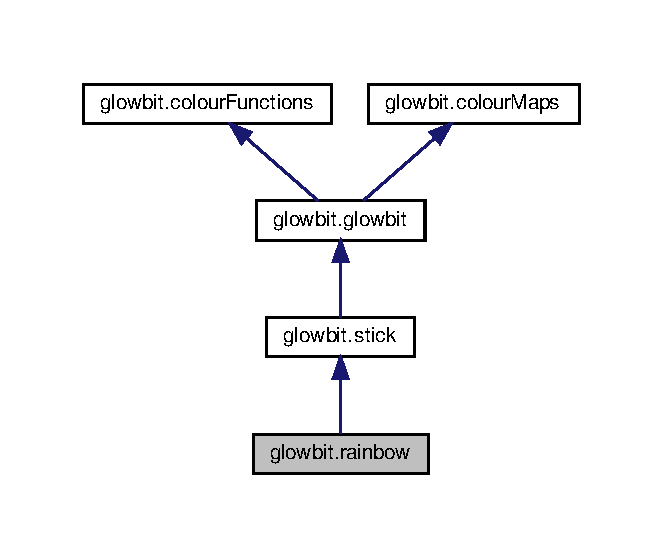
\includegraphics[width=318pt]{classglowbit_1_1rainbow__inherit__graph}
\end{center}
\end{figure}


Collaboration diagram for glowbit.\+rainbow\+:\nopagebreak
\begin{figure}[H]
\begin{center}
\leavevmode
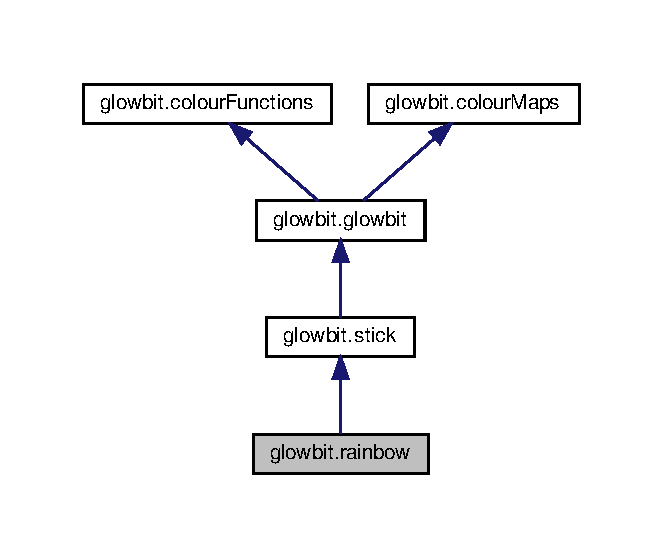
\includegraphics[width=318pt]{classglowbit_1_1rainbow__coll__graph}
\end{center}
\end{figure}
\subsection*{Public Member Functions}
\begin{DoxyCompactItemize}
\item 
def \hyperlink{classglowbit_1_1rainbow_ab1af2d27c10f3ffba7b3ce955cb6229f}{\+\_\+\+\_\+init\+\_\+\+\_\+} (self, num\+L\+E\+Ds=13, pin=18, brightness=40, rate\+Limit\+F\+PS=60, sm=0)
\begin{DoxyCompactList}\small\item\em Initialisation routine for Glow\+Bit rainbow modules. \end{DoxyCompactList}\item 
def \hyperlink{classglowbit_1_1rainbow_a0940825ae934617f95b96e472923f07a}{pixel\+Set\+Angle} (self, angle, colour)
\begin{DoxyCompactList}\small\item\em Sets the colour of a pixel on the Glow\+Bit Rainbow, addressed by its angle label. \end{DoxyCompactList}\item 
def \hyperlink{classglowbit_1_1rainbow_af03e480ce6a5d27780268b242a3fdfa7}{draw\+Rainbow} (self, offset=0)
\begin{DoxyCompactList}\small\item\em Colours each pixel to display a rainbow spectrum. \end{DoxyCompactList}\item 
def \hyperlink{classglowbit_1_1rainbow_ae693f9ccb27c683ee6d69728e8f9266f}{demo} (self)
\begin{DoxyCompactList}\small\item\em Displays a rainbow animation in an infinite loop. \end{DoxyCompactList}\end{DoxyCompactItemize}
\subsection*{Additional Inherited Members}


\subsection{Detailed Description}
The class specific to the Glow\+Bit Rainbow. 

This class inherits all the functionality of the Glow\+Bit Stick and extends it with Rainbow-\/specific methods. 

\subsection{Constructor \& Destructor Documentation}
\mbox{\Hypertarget{classglowbit_1_1rainbow_ab1af2d27c10f3ffba7b3ce955cb6229f}\label{classglowbit_1_1rainbow_ab1af2d27c10f3ffba7b3ce955cb6229f}} 
\index{glowbit\+::rainbow@{glowbit\+::rainbow}!\+\_\+\+\_\+init\+\_\+\+\_\+@{\+\_\+\+\_\+init\+\_\+\+\_\+}}
\index{\+\_\+\+\_\+init\+\_\+\+\_\+@{\+\_\+\+\_\+init\+\_\+\+\_\+}!glowbit\+::rainbow@{glowbit\+::rainbow}}
\subsubsection{\texorpdfstring{\+\_\+\+\_\+init\+\_\+\+\_\+()}{\_\_init\_\_()}}
{\footnotesize\ttfamily def glowbit.\+rainbow.\+\_\+\+\_\+init\+\_\+\+\_\+ (\begin{DoxyParamCaption}\item[{}]{self,  }\item[{}]{num\+L\+E\+Ds = {\ttfamily 13},  }\item[{}]{pin = {\ttfamily 18},  }\item[{}]{brightness = {\ttfamily 40},  }\item[{}]{rate\+Limit\+F\+PS = {\ttfamily 60},  }\item[{}]{sm = {\ttfamily 0} }\end{DoxyParamCaption})}



Initialisation routine for Glow\+Bit rainbow modules. 


\begin{DoxyParams}{Parameters}
{\em num\+L\+E\+Ds} & The total number of L\+E\+Ds. Should be set to 13 $\ast$ (the number of tiled modules). \\
\hline
{\em pin} & The G\+P\+IO pin connected to the Glow\+Bit Rainbow module. Defaults to 18 as that pin is compatible with the Raspberry Pi and Raspberry Pi Pico. Any pin can be used on the Raspberry Pi Pico, only pins 18 and 12 are valid on the Raspberry Pi. \\
\hline
{\em brightness} & The relative brightness of the L\+E\+Ds. Colours drawn to the internal buffer should be in the range \mbox{[}0,255\mbox{]} and the brightness parameter scales this value before drawing to the physical display. If brightness is an integer it should be in the range \mbox{[}0,255\mbox{]}. If brightness is floating point it is assumed to be in the range \mbox{[}0,1.\+0\mbox{]}. \\
\hline
{\em rate\+Limit\+F\+PS} & The maximum frame rate of the display in frames per second. The pixels\+Show() function blocks to enforce this limit. \\
\hline
\end{DoxyParams}


\subsection{Member Function Documentation}
\mbox{\Hypertarget{classglowbit_1_1rainbow_ae693f9ccb27c683ee6d69728e8f9266f}\label{classglowbit_1_1rainbow_ae693f9ccb27c683ee6d69728e8f9266f}} 
\index{glowbit\+::rainbow@{glowbit\+::rainbow}!demo@{demo}}
\index{demo@{demo}!glowbit\+::rainbow@{glowbit\+::rainbow}}
\subsubsection{\texorpdfstring{demo()}{demo()}}
{\footnotesize\ttfamily def glowbit.\+rainbow.\+demo (\begin{DoxyParamCaption}\item[{}]{self }\end{DoxyParamCaption})}



Displays a rainbow animation in an infinite loop. 

This method demonstrates the use of \hyperlink{classglowbit_1_1rainbow_af03e480ce6a5d27780268b242a3fdfa7}{draw\+Rainbow()}. \mbox{\Hypertarget{classglowbit_1_1rainbow_af03e480ce6a5d27780268b242a3fdfa7}\label{classglowbit_1_1rainbow_af03e480ce6a5d27780268b242a3fdfa7}} 
\index{glowbit\+::rainbow@{glowbit\+::rainbow}!draw\+Rainbow@{draw\+Rainbow}}
\index{draw\+Rainbow@{draw\+Rainbow}!glowbit\+::rainbow@{glowbit\+::rainbow}}
\subsubsection{\texorpdfstring{draw\+Rainbow()}{drawRainbow()}}
{\footnotesize\ttfamily def glowbit.\+rainbow.\+draw\+Rainbow (\begin{DoxyParamCaption}\item[{}]{self,  }\item[{}]{offset = {\ttfamily 0} }\end{DoxyParamCaption})}



Colours each pixel to display a rainbow spectrum. 

This method calls pixels\+Show().


\begin{DoxyParams}{Parameters}
{\em offset} & A \char`\"{}phase\char`\"{} offset mapping \mbox{[}0,360\mbox{]} degrees to \mbox{[}0,255\mbox{]}. A value of 0 displays red at angle 0 and purple at angle 180. A modulo-\/255 operation is performed, allowing this value to be any integer. The rain\+Loop() method varies this value to display an animation. \\
\hline
\end{DoxyParams}
\mbox{\Hypertarget{classglowbit_1_1rainbow_a0940825ae934617f95b96e472923f07a}\label{classglowbit_1_1rainbow_a0940825ae934617f95b96e472923f07a}} 
\index{glowbit\+::rainbow@{glowbit\+::rainbow}!pixel\+Set\+Angle@{pixel\+Set\+Angle}}
\index{pixel\+Set\+Angle@{pixel\+Set\+Angle}!glowbit\+::rainbow@{glowbit\+::rainbow}}
\subsubsection{\texorpdfstring{pixel\+Set\+Angle()}{pixelSetAngle()}}
{\footnotesize\ttfamily def glowbit.\+rainbow.\+pixel\+Set\+Angle (\begin{DoxyParamCaption}\item[{}]{self,  }\item[{}]{angle,  }\item[{}]{colour }\end{DoxyParamCaption})}



Sets the colour of a pixel on the Glow\+Bit Rainbow, addressed by its angle label. 


\begin{DoxyParams}{Parameters}
{\em angle} & An integer number in degrees equal to an angle label on the Glow\+Bit Rainbow P\+CB. \\
\hline
{\em colour} & A 32-\/bit Glow\+Bit colour value \\
\hline
\end{DoxyParams}


The documentation for this class was generated from the following file\+:\begin{DoxyCompactItemize}
\item 
glowbit.\+py\end{DoxyCompactItemize}

\hypertarget{classglowbit_1_1glowbitMatrix_1_1raindrop}{}\section{glowbit.\+glowbit\+Matrix.\+raindrop Class Reference}
\label{classglowbit_1_1glowbitMatrix_1_1raindrop}\index{glowbit.\+glowbit\+Matrix.\+raindrop@{glowbit.\+glowbit\+Matrix.\+raindrop}}


A class used by the \hyperlink{classglowbit_1_1glowbitMatrix_a088608e2586a76f09eb7312f2155f0b8}{rain()} demonstration.  


\subsection*{Public Member Functions}
\begin{DoxyCompactItemize}
\item 
\mbox{\Hypertarget{classglowbit_1_1glowbitMatrix_1_1raindrop_a5368f364866f8e2bbbb430f7bce8909c}\label{classglowbit_1_1glowbitMatrix_1_1raindrop_a5368f364866f8e2bbbb430f7bce8909c}} 
def {\bfseries \+\_\+\+\_\+init\+\_\+\+\_\+} (self, x, speed)
\item 
\mbox{\Hypertarget{classglowbit_1_1glowbitMatrix_1_1raindrop_aeb03aa245ab1507c74474f6ed7918aa4}\label{classglowbit_1_1glowbitMatrix_1_1raindrop_aeb03aa245ab1507c74474f6ed7918aa4}} 
def {\bfseries update} (self)
\item 
\mbox{\Hypertarget{classglowbit_1_1glowbitMatrix_1_1raindrop_a8139214ebb75e44097147c61d254de5f}\label{classglowbit_1_1glowbitMatrix_1_1raindrop_a8139214ebb75e44097147c61d254de5f}} 
def {\bfseries getY} (self)
\end{DoxyCompactItemize}
\subsection*{Public Attributes}
\begin{DoxyCompactItemize}
\item 
\mbox{\Hypertarget{classglowbit_1_1glowbitMatrix_1_1raindrop_a4c481273b383e7ceed52eaa0f39a1a0a}\label{classglowbit_1_1glowbitMatrix_1_1raindrop_a4c481273b383e7ceed52eaa0f39a1a0a}} 
{\bfseries x}
\item 
\mbox{\Hypertarget{classglowbit_1_1glowbitMatrix_1_1raindrop_ade3f6775e6494d001f52e04ae5626fcb}\label{classglowbit_1_1glowbitMatrix_1_1raindrop_ade3f6775e6494d001f52e04ae5626fcb}} 
{\bfseries speed}
\item 
\mbox{\Hypertarget{classglowbit_1_1glowbitMatrix_1_1raindrop_a59a8135a4a81b2fa5f2cbfb225cf1575}\label{classglowbit_1_1glowbitMatrix_1_1raindrop_a59a8135a4a81b2fa5f2cbfb225cf1575}} 
{\bfseries y}
\end{DoxyCompactItemize}


\subsection{Detailed Description}
A class used by the \hyperlink{classglowbit_1_1glowbitMatrix_a088608e2586a76f09eb7312f2155f0b8}{rain()} demonstration. 

The documentation for this class was generated from the following file\+:\begin{DoxyCompactItemize}
\item 
glowbit.\+py\end{DoxyCompactItemize}

\hypertarget{classglowbit_1_1rp2}{}\section{glowbit.\+rp2 Class Reference}
\label{classglowbit_1_1rp2}\index{glowbit.\+rp2@{glowbit.\+rp2}}
\subsection*{Classes}
\begin{DoxyCompactItemize}
\item 
class \hyperlink{classglowbit_1_1rp2_1_1PIO}{P\+IO}
\end{DoxyCompactItemize}
\subsection*{Public Member Functions}
\begin{DoxyCompactItemize}
\item 
\mbox{\Hypertarget{classglowbit_1_1rp2_a321dce63b34c6d482a065b96bf1f5ab6}\label{classglowbit_1_1rp2_a321dce63b34c6d482a065b96bf1f5ab6}} 
def {\bfseries asm\+\_\+pio} (sideset\+\_\+init, out\+\_\+shiftdir, autopull, pull\+\_\+thresh)
\end{DoxyCompactItemize}


The documentation for this class was generated from the following file\+:\begin{DoxyCompactItemize}
\item 
glowbit.\+py\end{DoxyCompactItemize}

\hypertarget{classglowbit_1_1stick}{}\section{glowbit.\+stick Class Reference}
\label{classglowbit_1_1stick}\index{glowbit.\+stick@{glowbit.\+stick}}


Inheritance diagram for glowbit.\+stick\+:\nopagebreak
\begin{figure}[H]
\begin{center}
\leavevmode
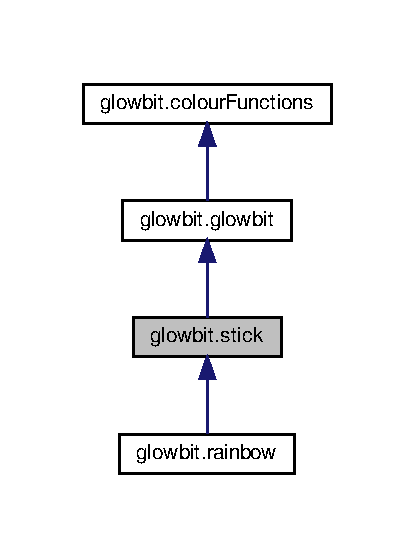
\includegraphics[width=199pt]{classglowbit_1_1stick__inherit__graph}
\end{center}
\end{figure}


Collaboration diagram for glowbit.\+stick\+:\nopagebreak
\begin{figure}[H]
\begin{center}
\leavevmode
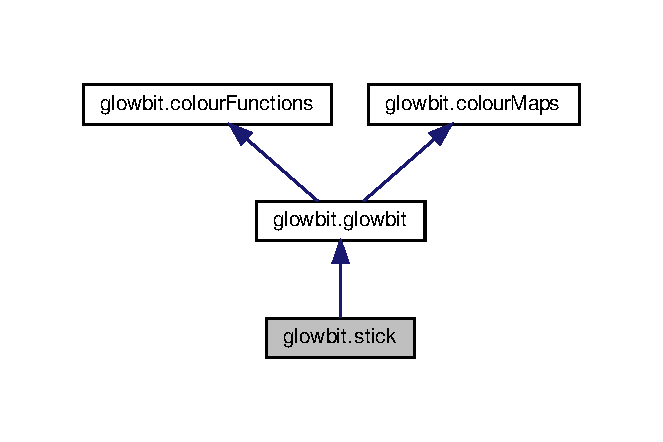
\includegraphics[width=199pt]{classglowbit_1_1stick__coll__graph}
\end{center}
\end{figure}
\subsection*{Classes}
\begin{DoxyCompactItemize}
\item 
class \hyperlink{classglowbit_1_1stick_1_1graph1D}{graph1D}
\begin{DoxyCompactList}\small\item\em One dimensional graph ofject for drawing a graph bar on a Glow\+Bit Stick display. \end{DoxyCompactList}\item 
class \hyperlink{classglowbit_1_1stick_1_1pulse}{pulse}
\begin{DoxyCompactList}\small\item\em A class for animating \char`\"{}pulses\char`\"{} which move down a Glow\+Bit stick. \end{DoxyCompactList}\end{DoxyCompactItemize}
\subsection*{Public Member Functions}
\begin{DoxyCompactItemize}
\item 
def \hyperlink{classglowbit_1_1stick_ac51b02c334481110558ac2f8c54938b8}{\+\_\+\+\_\+init\+\_\+\+\_\+} (self, num\+L\+E\+Ds=8, pin=18, brightness=20, rate\+Limit\+F\+PS=30, sm=0)
\begin{DoxyCompactList}\small\item\em Initialisation routine for Glow\+Bit stick modules and tiled arrays thereof. \end{DoxyCompactList}\item 
def \hyperlink{classglowbit_1_1stick_a14fb6c41aebc0b87595dde1ee4dd35a3}{add\+Pulse} (self, speed=100, colour=\mbox{[}0x\+F\+F\+F\+F\+F\+F\mbox{]}, index=0, colour\+Map=\+None)
\begin{DoxyCompactList}\small\item\em Add a pulse to the list of pulses. \end{DoxyCompactList}\item 
def \hyperlink{classglowbit_1_1stick_a84e72d81b9c96b1acb268b730866a8ea}{update\+Pulses} (self)
\begin{DoxyCompactList}\small\item\em Update the position of all pulses in self.\+pulses\mbox{[}\mbox{]} and draw them to the internal buffer. \end{DoxyCompactList}\item 
def \hyperlink{classglowbit_1_1stick_acde1622da63c602b209a608384cb6020}{update\+Graph1D} (self, graph, value)
\begin{DoxyCompactList}\small\item\em Updates a \hyperlink{classglowbit_1_1stick_1_1graph1D}{graph1D} object, drawing it to the display. \end{DoxyCompactList}\item 
def \hyperlink{classglowbit_1_1stick_a232b27f2f0e1c27787e6a584a05fc34c}{fill\+Slice} (self, i=0, j=-\/1, colour=0x\+F\+F\+F\+F\+F\+F)
\begin{DoxyCompactList}\small\item\em Fill a \char`\"{}slice\char`\"{} of the Glow\+Bit stick\textquotesingle{}s pixels with a solid colour. \end{DoxyCompactList}\item 
def \hyperlink{classglowbit_1_1stick_a1ea899a8e5ed6f4c24662853cb9a767d}{pulse\+Demo} (self, iters=100)
\begin{DoxyCompactList}\small\item\em A demonstration of the use of \char`\"{}pulse\char`\"{} objects. \end{DoxyCompactList}\item 
def \hyperlink{classglowbit_1_1stick_a7f45fb8bf324841b710a215b1b2e3a1c}{graph\+Demo} (self, iters=3)
\begin{DoxyCompactList}\small\item\em A demonstration of the use of \char`\"{}graph1\+D\char`\"{} objects. \end{DoxyCompactList}\item 
def \hyperlink{classglowbit_1_1stick_a26eedb25d40d67d1e2ca786a7b8eb8b0}{slice\+Demo} (self)
\begin{DoxyCompactList}\small\item\em A Demonstration of the use of the \char`\"{}fill\+Slice\char`\"{} method. \end{DoxyCompactList}\end{DoxyCompactItemize}
\subsection*{Public Attributes}
\begin{DoxyCompactItemize}
\item 
\mbox{\Hypertarget{classglowbit_1_1stick_a4530fd2c3995bb62da692005599035ad}\label{classglowbit_1_1stick_a4530fd2c3995bb62da692005599035ad}} 
{\bfseries sm}
\item 
\mbox{\Hypertarget{classglowbit_1_1stick_adbc03d4d11fcf4ec9cd8c03be41eb930}\label{classglowbit_1_1stick_adbc03d4d11fcf4ec9cd8c03be41eb930}} 
{\bfseries pixels\+Show}
\item 
\mbox{\Hypertarget{classglowbit_1_1stick_ae4a58846999c9f0aa96217e845594c03}\label{classglowbit_1_1stick_ae4a58846999c9f0aa96217e845594c03}} 
{\bfseries ticks\+\_\+ms}
\item 
\mbox{\Hypertarget{classglowbit_1_1stick_a77c1f5290c6d77d290e69bd9d30cadb4}\label{classglowbit_1_1stick_a77c1f5290c6d77d290e69bd9d30cadb4}} 
{\bfseries num\+L\+E\+Ds}
\item 
\mbox{\Hypertarget{classglowbit_1_1stick_a1c76eaa77ff6a78ae391443553ca67cc}\label{classglowbit_1_1stick_a1c76eaa77ff6a78ae391443553ca67cc}} 
{\bfseries strip}
\item 
\mbox{\Hypertarget{classglowbit_1_1stick_a64532e9357fcfb4430767856da0a3442}\label{classglowbit_1_1stick_a64532e9357fcfb4430767856da0a3442}} 
{\bfseries last\+Frame\+\_\+ms}
\item 
\mbox{\Hypertarget{classglowbit_1_1stick_a7c9f9a5cc34ac7ffb8ad260984986184}\label{classglowbit_1_1stick_a7c9f9a5cc34ac7ffb8ad260984986184}} 
{\bfseries ar}
\item 
\mbox{\Hypertarget{classglowbit_1_1stick_abdc6873e1788abb8def8c918463ba6ec}\label{classglowbit_1_1stick_abdc6873e1788abb8def8c918463ba6ec}} 
{\bfseries dimmer\+\_\+ar}
\item 
\mbox{\Hypertarget{classglowbit_1_1stick_a9412ada64a4c63191ca4c8b51c54c521}\label{classglowbit_1_1stick_a9412ada64a4c63191ca4c8b51c54c521}} 
{\bfseries rate\+Limit}
\item 
\mbox{\Hypertarget{classglowbit_1_1stick_af8d8ebbc0e29ecaacce4e1b04abf60dc}\label{classglowbit_1_1stick_af8d8ebbc0e29ecaacce4e1b04abf60dc}} 
{\bfseries brightness}
\item 
\mbox{\Hypertarget{classglowbit_1_1stick_a4c7704f407b6ee9f28136cb39f235cf6}\label{classglowbit_1_1stick_a4c7704f407b6ee9f28136cb39f235cf6}} 
{\bfseries pulses}
\end{DoxyCompactItemize}
\subsection*{Additional Inherited Members}


\subsection{Constructor \& Destructor Documentation}
\mbox{\Hypertarget{classglowbit_1_1stick_ac51b02c334481110558ac2f8c54938b8}\label{classglowbit_1_1stick_ac51b02c334481110558ac2f8c54938b8}} 
\index{glowbit\+::stick@{glowbit\+::stick}!\+\_\+\+\_\+init\+\_\+\+\_\+@{\+\_\+\+\_\+init\+\_\+\+\_\+}}
\index{\+\_\+\+\_\+init\+\_\+\+\_\+@{\+\_\+\+\_\+init\+\_\+\+\_\+}!glowbit\+::stick@{glowbit\+::stick}}
\subsubsection{\texorpdfstring{\+\_\+\+\_\+init\+\_\+\+\_\+()}{\_\_init\_\_()}}
{\footnotesize\ttfamily def glowbit.\+stick.\+\_\+\+\_\+init\+\_\+\+\_\+ (\begin{DoxyParamCaption}\item[{}]{self,  }\item[{}]{num\+L\+E\+Ds = {\ttfamily 8},  }\item[{}]{pin = {\ttfamily 18},  }\item[{}]{brightness = {\ttfamily 20},  }\item[{}]{rate\+Limit\+F\+PS = {\ttfamily 30},  }\item[{}]{sm = {\ttfamily 0} }\end{DoxyParamCaption})}



Initialisation routine for Glow\+Bit stick modules and tiled arrays thereof. 


\begin{DoxyParams}{Parameters}
{\em num\+L\+E\+Ds} & The total number of L\+E\+Ds. Should be set to 8 $\ast$ (the number of tiled modules). \\
\hline
{\em pin} & The G\+P\+IO pin connected to the Glow\+Bit stick module. Defaults to 18 as that pin is compatible with the Raspberry Pi and Raspberry Pi Pico. \\
\hline
{\em brightness} & The relative brightness of the L\+E\+Ds. Colours drawn to the internal buffer should be in the range \mbox{[}0,255\mbox{]} and the brightness parameter scales this value before drawing to the physical display. If brightness is an integer it should be in the range \mbox{[}0,255\mbox{]}. If brightness is floating point it is assumed to be in the range \mbox{[}0,1.\+0\mbox{]}. \\
\hline
{\em rate\+Limit\+F\+PS} & The maximum frame rate of the display in frames per second. The pixels\+Show() function blocks to enforce this limit. \\
\hline
{\em sm} & (Raspberry Pi Pico only) The P\+IO state machine to generate the Glow\+Bit data stream. Each connected Glow\+Bit display chain requires a unique state machine. Valid values are in the range \mbox{[}0,7\mbox{]}. \\
\hline
\end{DoxyParams}


\subsection{Member Function Documentation}
\mbox{\Hypertarget{classglowbit_1_1stick_a14fb6c41aebc0b87595dde1ee4dd35a3}\label{classglowbit_1_1stick_a14fb6c41aebc0b87595dde1ee4dd35a3}} 
\index{glowbit\+::stick@{glowbit\+::stick}!add\+Pulse@{add\+Pulse}}
\index{add\+Pulse@{add\+Pulse}!glowbit\+::stick@{glowbit\+::stick}}
\subsubsection{\texorpdfstring{add\+Pulse()}{addPulse()}}
{\footnotesize\ttfamily def glowbit.\+stick.\+add\+Pulse (\begin{DoxyParamCaption}\item[{}]{self,  }\item[{}]{speed = {\ttfamily 100},  }\item[{}]{colour = {\ttfamily \mbox{[}0xFFFFFF\mbox{]}},  }\item[{}]{index = {\ttfamily 0},  }\item[{}]{colour\+Map = {\ttfamily None} }\end{DoxyParamCaption})}



Add a pulse to the list of pulses. 


\begin{DoxyParams}{Parameters}
{\em speed} & The speed of the pulse in units of (pixels moved per frame) $\ast$ 100. A value of 100 means the pulse will move 1 pixels per frame. A speed of 1 will move a pulse 1 pixel every 100 frames. Speed can be positive or negative to allow pulses to move in either direction. \\
\hline
{\em colour} & A list of 32-\/bit Glow\+Bit colours for the pulse. The pulse will have a width equal to the number of elements in this list. A list entry of -\/1 will have the colour set by a colour map function. \\
\hline
{\em index} & The initial index of the pulse. Generally recommended to set to 0 if speed $>$ 0 and num\+L\+E\+Ds if speed $<$ 0. \\
\hline
{\em colour\+Map} & Either the string \char`\"{}\+Solid\char`\"{} or \char`\"{}\+Rainbow\char`\"{} or a custom function pointer. Custom functions must take the positional arguments\+: colour\+Map\+Function(self, index, min\+Index, max\+Index). When calling colour map functions \hyperlink{classglowbit_1_1stick_a84e72d81b9c96b1acb268b730866a8ea}{update\+Pulses()} sets min\+Index to 0 and max\+Index to num\+L\+E\+Ds. \\
\hline
\end{DoxyParams}
\mbox{\Hypertarget{classglowbit_1_1stick_a232b27f2f0e1c27787e6a584a05fc34c}\label{classglowbit_1_1stick_a232b27f2f0e1c27787e6a584a05fc34c}} 
\index{glowbit\+::stick@{glowbit\+::stick}!fill\+Slice@{fill\+Slice}}
\index{fill\+Slice@{fill\+Slice}!glowbit\+::stick@{glowbit\+::stick}}
\subsubsection{\texorpdfstring{fill\+Slice()}{fillSlice()}}
{\footnotesize\ttfamily def glowbit.\+stick.\+fill\+Slice (\begin{DoxyParamCaption}\item[{}]{self,  }\item[{}]{i = {\ttfamily 0},  }\item[{}]{j = {\ttfamily -\/1},  }\item[{}]{colour = {\ttfamily 0xFFFFFF} }\end{DoxyParamCaption})}



Fill a \char`\"{}slice\char`\"{} of the Glow\+Bit stick\textquotesingle{}s pixels with a solid colour. 

By default it will fill the entire display with a solid colour.


\begin{DoxyParams}{Parameters}
{\em i} & The minimum index to fill \\
\hline
{\em j} & The maximum index to fill \\
\hline
{\em colour} & A 32-\/bit Glow\+Bit colour value \\
\hline
\end{DoxyParams}
\mbox{\Hypertarget{classglowbit_1_1stick_a7f45fb8bf324841b710a215b1b2e3a1c}\label{classglowbit_1_1stick_a7f45fb8bf324841b710a215b1b2e3a1c}} 
\index{glowbit\+::stick@{glowbit\+::stick}!graph\+Demo@{graph\+Demo}}
\index{graph\+Demo@{graph\+Demo}!glowbit\+::stick@{glowbit\+::stick}}
\subsubsection{\texorpdfstring{graph\+Demo()}{graphDemo()}}
{\footnotesize\ttfamily def glowbit.\+stick.\+graph\+Demo (\begin{DoxyParamCaption}\item[{}]{self,  }\item[{}]{iters = {\ttfamily 3} }\end{DoxyParamCaption})}



A demonstration of the use of \char`\"{}graph1\+D\char`\"{} objects. 

This demonstration alternates between drawing two graphs with different colour maps; one with the \char`\"{}\+Rainbow\char`\"{} map, covering the full colour wheel, and another of solid white. 
\begin{DoxyParams}{Parameters}
{\em iters} & The number of times both graphs are drawn. \\
\hline
\end{DoxyParams}
\mbox{\Hypertarget{classglowbit_1_1stick_a1ea899a8e5ed6f4c24662853cb9a767d}\label{classglowbit_1_1stick_a1ea899a8e5ed6f4c24662853cb9a767d}} 
\index{glowbit\+::stick@{glowbit\+::stick}!pulse\+Demo@{pulse\+Demo}}
\index{pulse\+Demo@{pulse\+Demo}!glowbit\+::stick@{glowbit\+::stick}}
\subsubsection{\texorpdfstring{pulse\+Demo()}{pulseDemo()}}
{\footnotesize\ttfamily def glowbit.\+stick.\+pulse\+Demo (\begin{DoxyParamCaption}\item[{}]{self,  }\item[{}]{iters = {\ttfamily 100} }\end{DoxyParamCaption})}



A demonstration of the use of \char`\"{}pulse\char`\"{} objects. 

The pulse traveling \char`\"{}up\char`\"{} the stick is drawn with default arguments\+: a single white pixel

The pulse returning \char`\"{}down\char`\"{} the stick is drawn with a 3-\/pixel list of colours. The first and last are coloured with the \char`\"{}\+Rainbow\char`\"{} colour map, changing colour with pixel index, while the middle is white.


\begin{DoxyParams}{Parameters}
{\em iters} & The number of frames which are drawn before returning. \\
\hline
\end{DoxyParams}
\mbox{\Hypertarget{classglowbit_1_1stick_a26eedb25d40d67d1e2ca786a7b8eb8b0}\label{classglowbit_1_1stick_a26eedb25d40d67d1e2ca786a7b8eb8b0}} 
\index{glowbit\+::stick@{glowbit\+::stick}!slice\+Demo@{slice\+Demo}}
\index{slice\+Demo@{slice\+Demo}!glowbit\+::stick@{glowbit\+::stick}}
\subsubsection{\texorpdfstring{slice\+Demo()}{sliceDemo()}}
{\footnotesize\ttfamily def glowbit.\+stick.\+slice\+Demo (\begin{DoxyParamCaption}\item[{}]{self }\end{DoxyParamCaption})}



A Demonstration of the use of the \char`\"{}fill\+Slice\char`\"{} method. 

Animates a red, green, and blue slice \char`\"{}moving\char`\"{} down the Glow\+Bit Stick display.

The number of iterations is fixed due to the bit shift operation being used to change colour. \mbox{\Hypertarget{classglowbit_1_1stick_acde1622da63c602b209a608384cb6020}\label{classglowbit_1_1stick_acde1622da63c602b209a608384cb6020}} 
\index{glowbit\+::stick@{glowbit\+::stick}!update\+Graph1D@{update\+Graph1D}}
\index{update\+Graph1D@{update\+Graph1D}!glowbit\+::stick@{glowbit\+::stick}}
\subsubsection{\texorpdfstring{update\+Graph1\+D()}{updateGraph1D()}}
{\footnotesize\ttfamily def glowbit.\+stick.\+update\+Graph1D (\begin{DoxyParamCaption}\item[{}]{self,  }\item[{}]{graph,  }\item[{}]{value }\end{DoxyParamCaption})}



Updates a \hyperlink{classglowbit_1_1stick_1_1graph1D}{graph1D} object, drawing it to the display. 

If the \hyperlink{classglowbit_1_1stick_1_1graph1D}{graph1D} object was created with \char`\"{}update = True\char`\"{} this function will call pixels\+Show() to update the physical display before returning.


\begin{DoxyParams}{Parameters}
{\em graph} & A \hyperlink{classglowbit_1_1stick_1_1graph1D}{graph1D} object as returned by \hyperlink{classglowbit_1_1stick_1_1graph1D}{stick.\+graph1D} \\
\hline
{\em value} & The numerical value to plot on the graph \\
\hline
\end{DoxyParams}
\mbox{\Hypertarget{classglowbit_1_1stick_a84e72d81b9c96b1acb268b730866a8ea}\label{classglowbit_1_1stick_a84e72d81b9c96b1acb268b730866a8ea}} 
\index{glowbit\+::stick@{glowbit\+::stick}!update\+Pulses@{update\+Pulses}}
\index{update\+Pulses@{update\+Pulses}!glowbit\+::stick@{glowbit\+::stick}}
\subsubsection{\texorpdfstring{update\+Pulses()}{updatePulses()}}
{\footnotesize\ttfamily def glowbit.\+stick.\+update\+Pulses (\begin{DoxyParamCaption}\item[{}]{self }\end{DoxyParamCaption})}



Update the position of all pulses in self.\+pulses\mbox{[}\mbox{]} and draw them to the internal buffer. 

A call to pixels\+Show() must be done manually to update the physical L\+E\+Ds. 

The documentation for this class was generated from the following file\+:\begin{DoxyCompactItemize}
\item 
glowbit.\+py\end{DoxyCompactItemize}

\hypertarget{classglowbit_1_1matrix8x8_1_1textScroll}{}\section{glowbit.\+matrix8x8.\+text\+Scroll Class Reference}
\label{classglowbit_1_1matrix8x8_1_1textScroll}\index{glowbit.\+matrix8x8.\+text\+Scroll@{glowbit.\+matrix8x8.\+text\+Scroll}}
\subsection*{Public Member Functions}
\begin{DoxyCompactItemize}
\item 
\mbox{\Hypertarget{classglowbit_1_1matrix8x8_1_1textScroll_a4249d0c715faf3146f900ef070fc0360}\label{classglowbit_1_1matrix8x8_1_1textScroll_a4249d0c715faf3146f900ef070fc0360}} 
def {\bfseries \+\_\+\+\_\+init\+\_\+\+\_\+} (self, string, y=0, x=0, colour=0x\+F\+F\+F\+F\+F\+F, bg\+Colour=0)
\end{DoxyCompactItemize}
\subsection*{Public Attributes}
\begin{DoxyCompactItemize}
\item 
\mbox{\Hypertarget{classglowbit_1_1matrix8x8_1_1textScroll_a312c5b72b8ae76c6a04be069ec4167a3}\label{classglowbit_1_1matrix8x8_1_1textScroll_a312c5b72b8ae76c6a04be069ec4167a3}} 
{\bfseries x}
\item 
\mbox{\Hypertarget{classglowbit_1_1matrix8x8_1_1textScroll_a6e7ff4ac73a3434911cb92b7093032a0}\label{classglowbit_1_1matrix8x8_1_1textScroll_a6e7ff4ac73a3434911cb92b7093032a0}} 
{\bfseries y}
\item 
\mbox{\Hypertarget{classglowbit_1_1matrix8x8_1_1textScroll_aaf894a77ea70a49cedf7d0de28c1deb8}\label{classglowbit_1_1matrix8x8_1_1textScroll_aaf894a77ea70a49cedf7d0de28c1deb8}} 
{\bfseries colour}
\item 
\mbox{\Hypertarget{classglowbit_1_1matrix8x8_1_1textScroll_ac99afe118a82f3fc6ebcd09ce1ce2613}\label{classglowbit_1_1matrix8x8_1_1textScroll_ac99afe118a82f3fc6ebcd09ce1ce2613}} 
{\bfseries bg\+Colour}
\item 
\mbox{\Hypertarget{classglowbit_1_1matrix8x8_1_1textScroll_aa4cb9f51546632a1c6b82c425ca80a7f}\label{classglowbit_1_1matrix8x8_1_1textScroll_aa4cb9f51546632a1c6b82c425ca80a7f}} 
{\bfseries string}
\end{DoxyCompactItemize}


The documentation for this class was generated from the following file\+:\begin{DoxyCompactItemize}
\item 
glowbit.\+py\end{DoxyCompactItemize}

\hypertarget{classglowbit_1_1triangle}{}\section{glowbit.\+triangle Class Reference}
\label{classglowbit_1_1triangle}\index{glowbit.\+triangle@{glowbit.\+triangle}}


Class for driving triangular Glow\+Bit modules.  




Inheritance diagram for glowbit.\+triangle\+:\nopagebreak
\begin{figure}[H]
\begin{center}
\leavevmode
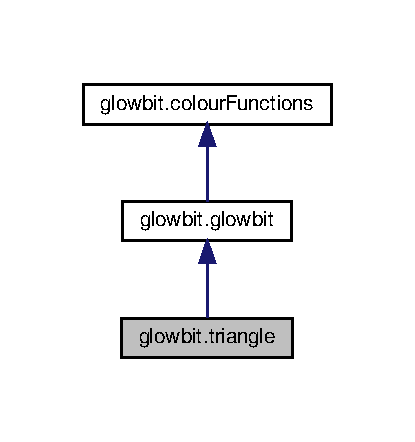
\includegraphics[width=318pt]{classglowbit_1_1triangle__inherit__graph}
\end{center}
\end{figure}


Collaboration diagram for glowbit.\+triangle\+:\nopagebreak
\begin{figure}[H]
\begin{center}
\leavevmode
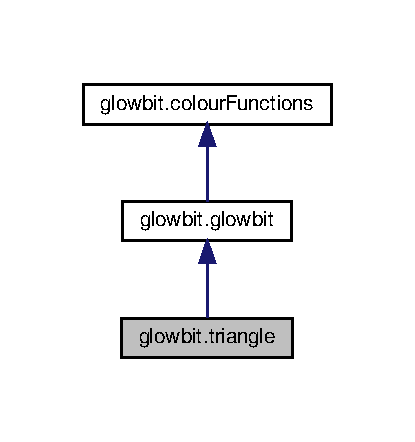
\includegraphics[width=318pt]{classglowbit_1_1triangle__coll__graph}
\end{center}
\end{figure}
\subsection*{Public Member Functions}
\begin{DoxyCompactItemize}
\item 
def \hyperlink{classglowbit_1_1triangle_aa9ff905dd6cde53bf8a39b3f8cb9482f}{\+\_\+\+\_\+init\+\_\+\+\_\+} (self, num\+Tris=1, L\+E\+Ds\+Per\+Tri=6, pin=18, brightness=20, rate\+Limit\+F\+PS=20, sm=0)
\begin{DoxyCompactList}\small\item\em Initialisation routine for triangular Glow\+Bit modules and tiled arrays thereof. \end{DoxyCompactList}\item 
def \hyperlink{classglowbit_1_1triangle_a26f35bf61d507d755ce039f4a0210c08}{fill\+Tri} (self, tri, colour)
\begin{DoxyCompactList}\small\item\em Fills all L\+E\+Ds on a given triangle with the same colour. \end{DoxyCompactList}\item 
\mbox{\Hypertarget{classglowbit_1_1triangle_a92bbeb798c85640681325d3d9654fefc}\label{classglowbit_1_1triangle_a92bbeb798c85640681325d3d9654fefc}} 
def \hyperlink{classglowbit_1_1triangle_a92bbeb798c85640681325d3d9654fefc}{demo} (self)
\begin{DoxyCompactList}\small\item\em Displays a simple demo pattern. \end{DoxyCompactList}\end{DoxyCompactItemize}
\subsection*{Public Attributes}
\begin{DoxyCompactItemize}
\item 
\mbox{\Hypertarget{classglowbit_1_1triangle_a826d6fe21b7e8fda3ad780fc83d83660}\label{classglowbit_1_1triangle_a826d6fe21b7e8fda3ad780fc83d83660}} 
{\bfseries sm}
\item 
\mbox{\Hypertarget{classglowbit_1_1triangle_ae8c7b20c01f071d0cc9bae97f414c2cf}\label{classglowbit_1_1triangle_ae8c7b20c01f071d0cc9bae97f414c2cf}} 
{\bfseries pixels\+Show}
\item 
\mbox{\Hypertarget{classglowbit_1_1triangle_adea9ee1f6a2446546c62847f705071c3}\label{classglowbit_1_1triangle_adea9ee1f6a2446546c62847f705071c3}} 
{\bfseries ticks\+\_\+ms}
\item 
\mbox{\Hypertarget{classglowbit_1_1triangle_ac6716c3af9a0c7928e5ef26507e9d07d}\label{classglowbit_1_1triangle_ac6716c3af9a0c7928e5ef26507e9d07d}} 
{\bfseries L\+E\+Ds\+Per\+Tri}
\item 
\mbox{\Hypertarget{classglowbit_1_1triangle_ac49c332e3aaaf1c4a1c909dee4b6cc2f}\label{classglowbit_1_1triangle_ac49c332e3aaaf1c4a1c909dee4b6cc2f}} 
{\bfseries num\+L\+E\+Ds}
\item 
\mbox{\Hypertarget{classglowbit_1_1triangle_a3e7ae1193100b0816a83b715f6862ab7}\label{classglowbit_1_1triangle_a3e7ae1193100b0816a83b715f6862ab7}} 
{\bfseries num\+Tris}
\item 
\mbox{\Hypertarget{classglowbit_1_1triangle_a91f7966af0e17ef99e68ec8cf672e313}\label{classglowbit_1_1triangle_a91f7966af0e17ef99e68ec8cf672e313}} 
{\bfseries strip}
\item 
\mbox{\Hypertarget{classglowbit_1_1triangle_a1cd0a82b5c269c019c37f7bb2892680d}\label{classglowbit_1_1triangle_a1cd0a82b5c269c019c37f7bb2892680d}} 
{\bfseries ar}
\item 
\mbox{\Hypertarget{classglowbit_1_1triangle_afadb993656f4bb24c5923a6e677f214b}\label{classglowbit_1_1triangle_afadb993656f4bb24c5923a6e677f214b}} 
{\bfseries dimmer\+\_\+ar}
\item 
\mbox{\Hypertarget{classglowbit_1_1triangle_abb1773a93e2fafeae40f8a2cc4e77a81}\label{classglowbit_1_1triangle_abb1773a93e2fafeae40f8a2cc4e77a81}} 
{\bfseries rate\+Limit}
\item 
\mbox{\Hypertarget{classglowbit_1_1triangle_ad55aff3faee32703d2dec714a5c42de5}\label{classglowbit_1_1triangle_ad55aff3faee32703d2dec714a5c42de5}} 
{\bfseries brightness}
\item 
\mbox{\Hypertarget{classglowbit_1_1triangle_a9b282fc22b8e029983f33c24f1a4ca01}\label{classglowbit_1_1triangle_a9b282fc22b8e029983f33c24f1a4ca01}} 
{\bfseries last\+Frame\+\_\+ms}
\end{DoxyCompactItemize}
\subsection*{Additional Inherited Members}


\subsection{Detailed Description}
Class for driving triangular Glow\+Bit modules. 

\subsection{Constructor \& Destructor Documentation}
\mbox{\Hypertarget{classglowbit_1_1triangle_aa9ff905dd6cde53bf8a39b3f8cb9482f}\label{classglowbit_1_1triangle_aa9ff905dd6cde53bf8a39b3f8cb9482f}} 
\index{glowbit\+::triangle@{glowbit\+::triangle}!\+\_\+\+\_\+init\+\_\+\+\_\+@{\+\_\+\+\_\+init\+\_\+\+\_\+}}
\index{\+\_\+\+\_\+init\+\_\+\+\_\+@{\+\_\+\+\_\+init\+\_\+\+\_\+}!glowbit\+::triangle@{glowbit\+::triangle}}
\subsubsection{\texorpdfstring{\+\_\+\+\_\+init\+\_\+\+\_\+()}{\_\_init\_\_()}}
{\footnotesize\ttfamily def glowbit.\+triangle.\+\_\+\+\_\+init\+\_\+\+\_\+ (\begin{DoxyParamCaption}\item[{}]{self,  }\item[{}]{num\+Tris = {\ttfamily 1},  }\item[{}]{L\+E\+Ds\+Per\+Tri = {\ttfamily 6},  }\item[{}]{pin = {\ttfamily 18},  }\item[{}]{brightness = {\ttfamily 20},  }\item[{}]{rate\+Limit\+F\+PS = {\ttfamily 20},  }\item[{}]{sm = {\ttfamily 0} }\end{DoxyParamCaption})}



Initialisation routine for triangular Glow\+Bit modules and tiled arrays thereof. 


\begin{DoxyParams}{Parameters}
{\em num\+Tris} & The number of triangle modules in the tiled array. \\
\hline
{\em L\+E\+Ds\+Per\+Tri} & The number of L\+E\+Ds on each triangular module. \\
\hline
{\em pin} & The G\+P\+IO pin connected to the Glow\+Bit stick module. Defaults to 18 as that pin is compatible with the Raspberry Pi and Raspberry Pi Pico. Any pin can be used on the Raspberry Pi Pico, only pins 18 and 12 are valid on the Raspberry Pi. \\
\hline
{\em brightness} & The relative brightness of the L\+E\+Ds. Colours drawn to the internal buffer should be in the range \mbox{[}0,255\mbox{]} and the brightness parameter scales this value before drawing to the physical display. If brightness is an integer it should be in the range \mbox{[}0,255\mbox{]}. If brightness is floating point it is assumed to be in the range \mbox{[}0,1.\+0\mbox{]}. \\
\hline
{\em rate\+Limit\+F\+PS} & The maximum frame rate of the display in frames per second. The pixels\+Show() function blocks to enforce this limit. \\
\hline
{\em sm} & (Raspberry Pi Pico only) The P\+IO state machine to generate the Glow\+Bit data stream. Each connected Glow\+Bit display chain requires a unique state machine. Valid values are in the range \mbox{[}0,7\mbox{]}. \\
\hline
\end{DoxyParams}


\subsection{Member Function Documentation}
\mbox{\Hypertarget{classglowbit_1_1triangle_a26f35bf61d507d755ce039f4a0210c08}\label{classglowbit_1_1triangle_a26f35bf61d507d755ce039f4a0210c08}} 
\index{glowbit\+::triangle@{glowbit\+::triangle}!fill\+Tri@{fill\+Tri}}
\index{fill\+Tri@{fill\+Tri}!glowbit\+::triangle@{glowbit\+::triangle}}
\subsubsection{\texorpdfstring{fill\+Tri()}{fillTri()}}
{\footnotesize\ttfamily def glowbit.\+triangle.\+fill\+Tri (\begin{DoxyParamCaption}\item[{}]{self,  }\item[{}]{tri,  }\item[{}]{colour }\end{DoxyParamCaption})}



Fills all L\+E\+Ds on a given triangle with the same colour. 


\begin{DoxyParams}{Parameters}
{\em tri} & The triangle to fill. The first triangle is addressed with 0. \\
\hline
{\em colour} & A 32-\/bit Glow\+Bit colour value \\
\hline
\end{DoxyParams}


The documentation for this class was generated from the following file\+:\begin{DoxyCompactItemize}
\item 
glowbit.\+py\end{DoxyCompactItemize}

%--- End generated contents ---

% Index
\backmatter
\newpage
\phantomsection
\clearemptydoublepage
\addcontentsline{toc}{chapter}{Index}
\printindex

\end{document}
